\documentclass[a4paper,11pt]{report}

% Fonts (XeTeX/Tectonic)
\usepackage{fontspec}
\usepackage{amsmath}
\defaultfontfeatures{Ligatures=TeX}

% Typography
\usepackage{microtype}
\usepackage{parskip}
\setlength{\emergencystretch}{3em}

% Tables and figures
\usepackage{longtable,booktabs,array,threeparttablex}
\usepackage{fancyvrb}
\DefineVerbatimEnvironment{Prompt}{Verbatim}{frame=single,fontsize=\small}
\usepackage{graphicx}
\usepackage{rotating} % sidewaysfigure: full-page landscape recognition matrix (0446)
\usepackage{pdfpages} % \includepdf: multi-page portrait recognition matrix (0503)
\usepackage{xcolor}

% Links
\usepackage{bookmark}
\usepackage{xurl}
\urlstyle{same}
\hypersetup{hidelinks}

\setcounter{secnumdepth}{3}

\title{AEDIST: AI for Energy Data, Information and Statistics\\
\large Rapport technique}
\author{Minh Ha-Duong\\CIRED -- CNRS}
\date{2026}

\usepackage[round,authoryear]{natbib}
\bibliographystyle{plainnat}

% Auto-generated by aedist.tabulate_macros — do not edit
\newcommand{\NumModelsTested}{86}
\newcommand{\NumCloudModels}{75}
\newcommand{\NumLocalModels}{11}
\newcommand{\NumRefPlants}{163}
\newcommand{\BestModelName}{Claude Opus 4.6 Tool}
\newcommand{\BestModelFOne}{98.2}
\newcommand{\BestModelFOneCI}{[98.2, 98.2]}
\newcommand{\BestLocalName}{Padme Qwen3.5 9B}
\newcommand{\BestLocalFOne}{59.5}
\newcommand{\MinBaselinePlants}{0}
\newcommand{\MaxBaselinePlants}{160}

\InputIfFileExists{inputs/generated/macros_census}{}{}
\InputIfFileExists{inputs/generated/macros_exp1_matrix}{}{}

\begin{document}

\maketitle
\setcounter{tocdepth}{2}
\tableofcontents

\begin{abstract}
Nous évaluons la capacité de l'IA à produire des statistiques énergétiques, en utilisant l'inventaire des centrales thermiques du Vietnam comme benchmark. Seize grands modèles de langage sont testés en requête directe puis en approche conversationnelle avec relances~; les résultats sont ensuite améliorés par Retrieval Augmented Generation (RAG) à partir de documents sources, et comparés aux données disponibles dans les graphes de connaissances globaux (OpenStreetMap, Wikidata, Diffbot, DBpedia).

Les LLM seuls retournent 30 à 40 centrales sur \NumRefPlants{} recensées~; l'approche RAG wholesale porte le meilleur résultat à 117 centrales (F1 = 71,8\,\%). La décomposition par type de combustible atteint un F1 moyen de 68,6\,\% [60,7--74,8\,\%, IC 95\,\%, $n=4$] pour 0,06~\$, avec un modèle open-weight. Les graphes globaux apportent des données complémentaires mais aucun n'est suffisant seul.

Ces résultats montrent qu'un pipeline RAG avec décomposition des requêtes récupère une part substantielle d'un inventaire expert pour un coût marginal, mais avec une variance inter-runs élevée. Le défi restant relève de l'ingénierie de la connaissance~: filtrage des hallucinations, résolution d'entités et traçabilité des sources.
\end{abstract}

\chapter{Introduction}

\section{Problématique}

Est-il possible de suivre la transition énergétique d'un pays qui ne dispose pas d'un office de statistique performant dans ce domaine, sur la base de sources ouvertes? La tâche est faisable par un expert~: pendant plusieurs années, nous avons maintenu des tables de référence des projets de génération électrique au Vietnam, qu'ils soient opérationnels, en construction ou planifiés \citep{NLN8GPNI}. Les types de combustible y sont classés selon les nomenclatures internationales~: codes IRES (ONU, 2011) pour les produits énergétiques, codes ISIC Rév.~4 pour les activités industrielles, et vecteurs PyPSA-Earth pour la modélisation des systèmes électriques.

Dans quelle mesure peut on automatiser ce processus avec les nouveaux outils de data science?
Ce rapport examine les conditions de création d'un système qui collectera et analysera les données disponibles sur le deep web en quasi temps-réel, et utilisera des outils AI ouverts, contrôlés et exécutés localement.

\section{Exemple introductif (février 2025)}

Quand on demande \emph{«~Quelle est la puissance installée des centrales électriques au Vietnam, par type de génération~?~»} un LLM est capable de répondre de mémoire un chiffre plausible. Par exemple «~Voici une estimation basée sur les informations accessibles jusqu'en 2023. Ces chiffres peuvent avoir légèrement changé selon les nouvelles installations ou les projets récents\ldots{} Charbon (centrales thermiques).. Puissance estimée: environ 25-30 GW...~» (GPT-4o le interrogé 10 février 2025). Le chiffre n'est ni très précis, ni très actuel.

Un système plus perfectionné peut rechercher des information sur le web, et faire une synthèse réfléchie des sources. Par exemple \emph{«~Voici la puissance installée des centrales électriques au Vietnam, par type de génération, basée sur les données disponibles: En 2019: Capacité totale installée: 55 489 MW. Charbon: 36,52\% (20 267 MW)\ldots{} en 2023: Capacité totale installée: 80 500 MW (estimation), Charbon: ~46,9\% (37 755 MW)...~»} (DeepSeek R1 avec Thinking et Search, même jour). Pour 2023 il a raisonné en croisant deux sources, l'une donnant les pourcentages et l'autre la capacité totale. Le système donne les sources, il semble plausible. Mais la réponse est fausse car les pourcentages décrivaient la production annuelle, alors qu'on a demandé des capacités. Or les centrales à charbon sont utilisées davantage d'heures par an que les autres sortes de centrales électriques (le Vietnam n'a pas de centrale nucléaire). C'est une erreur courante, les non spécialistes confondent souvent kW et kWh.

En tant qu'expert, je répondrais «~\emph{Selon le post du 7 janvier 2025 sur le fil LinkedIn de Cuong Tran Duc, expert crédible dans le domaine, La capacité totale fin 2024 était 82.387 MW dont charbon 26 757~MW...}~». Si on demande de mieux justifier l'information, je trouverais sur le site de la Vietnam Energy Association la provenance de l'information~: Vietnam Electricity Group, conférence du 6 janvier 2025 présentant les résultats 2024 et objectifs 2025 \citep{DVW38BYR}. Documenter la provenance des données n'est pas une fin en soi, cela permet de s'assurer que la source est la meilleure disponible et la plus à jour.

Cet exemple montre plusieurs limites des AI en février 2025. Non seulement elles n'ont pas une connaissance experte de ce sujet technique, mais leur veille actualisée n'est pas ciblée sur les sources pertinentes fiables. Au surplus, l'usage de grands LLM en ligne pose des problèmes de sécurité~: pérennité de la disponibilité de l'outil (obsolescence et changements d'API), contrôle du processus (la plupart des fournisseurs dégradent le service aux heures de pointe), contraintes de souveraineté (DeepSeek R1 est bloqué aux USA).

\section{Un problème difficile à bien résoudre}

La difficulté de l'exercice est multiple. Le \textbf{multilinguisme}~: il convient de traiter l'information dans sa langue originale, pour des pays en développement, et par exemple la toponymie des petits barrages dans les régions reculées peut utiliser des langues rares. La \textbf{temporalité}~: certains documents sont des plans que la progression des chantiers et les changements politiques remettent en question rapidement. La \textbf{technicité}~: une culture d'ingénieur est nécessaire (différence entre kW et kWh, entre MWth et MWe). La \textbf{multidisciplinarité}~: Suivre la transition énergétique exige de comprendre les enjeux géopolitiques, d'environnement, de développement, de commerce international, d'avoir des connaissances en business (rôle des Special Purpose Vehicles companies), ou encore en administration (rôle des plans de développement du secteur électrique).

Par exemple, dans le domaine de la production d'électricité, les inventaires nationaux de parc peuvent se faire à quatre niveaux de détail~: le complexe industriel (power center), la centrale thermique, les unités de production, et la turbine. Le complexe de Phú~Mỹ, parfois noté Phú Mỹ 1-4 voire Phu My 1-4 en version translittérée, ne compte pas moins de six centrales. Chacune compte une unité de génération, avec deux turbines à gaz et une à vapeur puisque ce sont des centrales à gaz à cycle combiné (TBKHH en Vietnamien, CCGT en anglais ou français d'affaires, CCG en français spécifique)~:

\begin{enumerate}
\item Phú Mỹ 1
\item Phú Mỹ 2-1
\item Phú Mỹ 2-1 extension
\item Phú Mỹ 2-2
\item Phú Mỹ 3
\item Phú Mỹ 4
\end{enumerate}

Les centrales 1, 2.1, 2.1 extension et4 sont à la Phu My Thermal Power Company, une filiale de EVN Genco 3, elle même filiale de EVN (anciennement Électricité du Vietnam). La centrale 3 a été construite par Siemens pour BP en 2024 avec une licence Build-Operate-Transfer de 20 ans, Sembcorp l'a transféré à EVN Genco 3 en 2024. La centrale 2-2 a été construite en 2005, est opérée par un consortium Franco-Japonais et a été retransférée au gouvernement vietnamien le 4 décembre 2024 \citep{UAWJD84R}.

De plus, une proposition de centrale Phú Mỹ 3.1 de 850 MW utilisant du LNG figure dans le Draft PDP8, Appendix 9.1, MOIT du 22 février 2021 (PDP signifie Power Development Plan). Elle est aussi évoquée dans un article rapportant des discussions entre le MOIT (le Ministère de l'Industrie et du Commerce, responsable du secteur de l'énergie) et la province de Ba Ria-Vung Tau le 7 janvier 2020. Elle n'a pas été retenue dans la version finale du PDP8. Un chercheur peut cependant attendre qu'elle figure à un inventaire des centrales historiques ou en projet~: la sur-proposition de centrales LNG lors de la préparation du PDP8 est un événement intéressant à bien des égards. On attend donc sept lignes pour Phú Mỹ 1-4 dans l'inventaire.

\section{Mais il existe des solutions}

Bien que difficile à réaliser parfaitement, les inventaires de moyens de génération sont d'une grande importance économique, technique et environnementale. Il existe donc des listes disponibles~: une compilée par nous même \citep{NLN8GPNI}, une page Wikipedia \citep{TQ8TFB8H} à laquelle nous avons beaucoup contribuée, la base de donnée ouverte Global Energy Monitor \citep{LCVI7NAT}, ainsi que les dataset en fichiers HDF5 utilisés dans les modèles comme pypsa-earth \citep{UMGUESAZ} et pypsa-vn \citep{VGASHFPT}. Il en existe d'autres, mais \citep{LYGDCQCL} montre que la qualité de l'information disponible en accès libre, même en combinant les diverses sources, n'atteignait pas celle de la base propriétaire S\&P Global Platts Power Plants.

Ce rapport ne prétend donc pas s'attaquer un problème original, il s'agit plutôt d'adopter un benchmark. La méthode consiste de comparer la performance de différents outils disponibles pour répondre à la question. On progressera du plus simple au plus sophistiqué, pour montrer les limites et tracer les contours de notre proposition. Le but est un système de suivi de la transition énergétique dans tous les pays, le cas des centrales thermiques au Viêtnam est une première marche.

Ce rapport explore la question au niveau faisabilité. L'optimisation du coût, du temps, ou l'automatisation complète n'est pas étudiée dans ce rapport~. On utilisera donc des LLM en ligne de grand taille -- typiquement 400B -- , même si le but ultérieur est d'utiliser des agents basés sur des modèles de taille plus modeste exécutés localement.

\section{Plan}

Ce rapport progresse du plus simple au plus sophistiqué. Le chapitre~\ref{chap:evaluation} évalue la capacité des LLM à produire des tables statistiques, d'abord en requête directe, puis par approche conversationnelle avec relances. Le chapitre~\ref{chap:rag} traite de la découverte des documents sources et de l'amélioration des résultats par Retrieval Augmented Generation (RAG). Le chapitre~\ref{chap:kg} examine l'apport des graphes de connaissances pour la traçabilité et la structuration des données. Le chapitre~\ref{chap:agents} évalue les systèmes multi-agents existants. Le chapitre~\ref{chap:architecture} propose une architecture hybride combinant ces approches. Le chapitre~\ref{chap:conclusion} dresse le bilan des résultats quantitatifs et évalue la faisabilité de l'approche.

\chapter{Évaluation des LLM}\label{chap:evaluation}

Ce chapitre évalue la capacité des grands modèles de langage à produire des tables statistiques au moyen de deux études préliminaires~: d'abord en requête directe (single-shot), puis par approche conversationnelle avec relances.

\section{Méthodologie}

On évalue la performance de différents modèles d'IA dans la production directe de données statistiques, sur la tâche d'inventaire des centrales thermiques du Vietnam. La méthodologie procède en trois temps~:

\begin{enumerate}
\item Sélection d'un échantillon diversifié de modèles, incluant des modèles de grande taille (400B+ paramètres) et des modèles plus modestes (70B).
\item Requête standardisée demandant une liste complète des centrales thermiques du Vietnam avec leurs caractéristiques techniques (Prompt~1 pour l'étude en requête directe, Prompt~2 avec relances pour l'étude conversationnelle).
\item Évaluation de l'exhaustivité des réponses par rapport à la page Wikipedia \citep{TQ8TFB8H} qui recense 88 centrales à charbon et 26 centrales à gaz.
\end{enumerate}

Texte de la requête initiale (\emph{Prompt~1})~:

\begin{Prompt}
Provide a table listing all thermal power plants in Vietnam, including their
fuel type (coal / local natural gas / imported LNG), construction stage,
connection date (observed or planned COD), province, and generation capacity
(in MWe). Format the response in CSV.
\end{Prompt}

\section{Étude préliminaire~: requête directe (single-shot)}\label{sec:exp1}

Les résultats sont loin de la qualité statistique. Les modèles flagship retournent entre 18 et 64 centrales~: R1-DeepSeek with search en trouve 64, Gemini-2-flash 41, Claude~3.5 Sonnet 38, GPT-4o 33. La performance est corrélée à la nouveauté des modèles.

On observe trois stratégies de réponse distinctes~: (a) fourniture de données étendues avec avertissements (Claude, GPT-4o), (b) fourniture d'une structure sans données incertaines (Mistral-Large-2), (c) conseils méthodologiques plutôt que données (Qwen-QwQ-32b-preview). Aucun modèle ne répond exactement à la question.

La limite de taille des réponses (4K--8K tokens) joue un rôle critique~: l'information demandée représente au minimum 2~267 tokens même avec des cellules vides, alors que notre table de référence \citep{NLN8GPNI} en compte 27~946. C'est d'autant plus un problème pour les modèles de raisonnement, qui allouent une partie du résultat à la réflexion.

% Auto-generated — do not edit
\begin{longtable}[]{@{}lrrrr@{}}
\caption{Model census: single-shot F1 scores (median of 3 runs)}\label{tab:census}\\
\toprule
Model & F1 & Precision & Recall & Matched \\
\midrule
\endhead
\bottomrule
\endlastfoot
Gemini-2.5-Flash-Lite & 95.3\% & 91.1\% & 100.0\% & 163/163 \\
GPT-5.4 & 63.6\% & 100.0\% & 46.6\% & 76/163 \\
GLM-5-Turbo & 60.1\% & 100.0\% & 42.9\% & 70/163 \\
Claude-Opus-4.6 & 58.3\% & 100.0\% & 41.1\% & 67/163 \\
GLM-4.7-Flash (L) & 57.6\% & 100.0\% & 40.5\% & 66/163 \\
Gemini-3-Flash-Preview & 56.4\% & 100.0\% & 39.3\% & 64/163 \\
Claude-Sonnet-4.6 & 53.8\% & 100.0\% & 36.8\% & 60/163 \\
Kimi-K2.5 & 53.1\% & 100.0\% & 36.2\% & 59/163 \\
Mistral-Small-2603 & 51.1\% & 100.0\% & 34.4\% & 56/163 \\
Qwen3.5-397b-A17b & 44.0\% & 100.0\% & 28.2\% & 46/163 \\
DeepSeek-V3.2 & 38.6\% & 100.0\% & 23.9\% & 39/163 \\
Qwen3.5-35b-A3b & 37.8\% & 100.0\% & 23.3\% & 38/163 \\
Mistral-Large-2512 & 37.0\% & 100.0\% & 22.7\% & 37/163 \\
Minimax-M2.7 & 35.4\% & 100.0\% & 21.5\% & 35/163 \\
Qwen3.5-9b (L) & 35.4\% & 100.0\% & 21.5\% & 35/163 \\
MiMo-V2-Flash & 32.8\% & 100.0\% & 19.6\% & 32/163 \\
MiMo-V2-Pro & 32.8\% & 100.0\% & 19.6\% & 32/163 \\
Qwen3.5-Plus-02-15 & 32.0\% & 100.0\% & 19.0\% & 31/163 \\
Qwen3.6-Plus-Preview-Free & 31.1\% & 100.0\% & 18.4\% & 30/163 \\
Mercury-2 & 27.5\% & 100.0\% & 16.0\% & 26/163 \\
Devstral-Small-2 (L) & 21.9\% & 100.0\% & 12.3\% & 20/163 \\
Qwen3.5-27b & 21.9\% & 100.0\% & 12.3\% & 20/163 \\
Nemotron-3-Nano (L) & 20.9\% & 100.0\% & 11.7\% & 19/163 \\
Qwen3.5-27b (L) & 20.9\% & 100.0\% & 11.7\% & 19/163 \\
Qwen3.5-35b (L) & 20.9\% & 100.0\% & 11.7\% & 19/163 \\
Nemotron-3-Nano-30b-A3b & 18.9\% & 100.0\% & 10.4\% & 17/163 \\
Seed-2.0-Lite & 13.7\% & 100.0\% & 7.4\% & 12/163 \\
Llama-4-Maverick & 9.4\% & 100.0\% & 4.9\% & 8/163 \\
Grok-4.20 & 2.4\% & 100.0\% & 1.2\% & 2/163 \\
GPT-5-Mini & 0.0\% & 0.0\% & 0.0\% & 0/0 \\
GPT-5-Nano & 0.0\% & 0.0\% & 0.0\% & 0/0 \\
Gemma4-26b (L) & 0.0\% & 0.0\% & 0.0\% & 0/0 \\
Gemma4-31b (L) & 0.0\% & 0.0\% & 0.0\% & 0/0 \\
Mistral-Small3.2 (L) & 0.0\% & 0.0\% & 0.0\% & 0/0 \\
Qwen3.5-122b-A10b & 0.0\% & 0.0\% & 0.0\% & 0/0 \\
\end{longtable}


\paragraph{Capture de l'intensité de raisonnement et variabilité interjournalière.}
La table~\ref{tab:exp1-reasoning-topup} prolonge la cohorte du 20~mai~2026 (16 modèles, $N{=}5$~répétitions) par une cohorte complémentaire du 21~mai~2026 ($N{\leq}3$) exécutée après le correctif de harnais PR\#379, qui rend visible le compteur \texttt{reasoning\_tokens} exposé par OpenRouter dans \texttt{completion\_tokens\_details}. Les deux cohortes partagent la même configuration d'appel (\texttt{model\_set}, prompt, température, \texttt{seed}, \texttt{system\_instruction}, \texttt{max\_tokens})~; seules diffèrent la date d'exécution et la version du harnais. Trois modèles présentent un écart $|\Delta\text{F1}| > 2\sigma_{\text{baseline}}$ entre les deux jours~: \emph{DeepSeek-V4-Pro} ($-0.185$, raisonnement intensif à 16~774~tokens), \emph{Qwen3.6-27b} ($+0.289$) et \emph{Qwen3.6-35b-A3b} ($+0.165$). Cette variabilité interjournalière, à configuration d'appel inchangée et à \texttt{seed=42}, illustre que les contrôles habituels (température nulle, \emph{seed} fixe) ne suffisent pas à neutraliser les déplacements silencieux côté fournisseur (routage, mise à jour de checkpoint). Le compteur \texttt{reasoning\_tokens} confirme par ailleurs deux régimes contrastés~: les modèles Anthropic et Mistral du panel ne rapportent aucun token de raisonnement, tandis que les modèles DeepSeek V4, Qwen3.6 et GPT-OSS en allouent entre quelques dizaines (déclaration \texttt{reasoning\_effort="minimal"}) et plus de 16~000.

% Auto-generated by aedist.tabulate_exp1_reasoning_topup — do not edit
\begin{table}[htbp]
\centering
\small
\caption{Experiment~1 results, pooled across the 2026-05-20 baseline ($N{\leq}5$) and a 2026-05-21 post-fix top-up cohort ($N{\leq}3$). The post-fix cohort captures \texttt{reasoning\_tokens} via the OpenRouter \texttt{completion\_tokens\_details} channel (PR\#379). $\Delta$F1 reports the interday shift in mean F1 (post-fix minus baseline). Models with $|\Delta\text{F1}|>2\sigma_{\text{baseline}}$ (boldface) showed a behaviour shift between cohorts and are noted in the discussion.}
\label{tab:exp1-reasoning-topup}
\begin{tabular}{lrrrrrr}
\toprule
Model & $N_{\text{base}}$ & $N_{\text{post}}$ & F1 baseline & F1 post-fix & $\Delta$F1 & Reasoning tokens* \\
\midrule
Claude-Haiku-4.5 & 5 & 3 & 0.189 & 0.189 & +0.000 & 0 \\
Claude-Opus-4.6 & 5 & 3 & 0.463\,$\pm$\,0.057 & 0.500\,$\pm$\,0.011 & +0.036 & 0 \\
Claude-Sonnet-4.6 & 5 & 3 & 0.420\,$\pm$\,0.065 & 0.479\,$\pm$\,0.004 & +0.059 & 0 \\
DeepSeek-V4-Flash & 5 & 2 & 0.448\,$\pm$\,0.263 & 0.446\,$\pm$\,0.131 & -0.002 & 775 \\
DeepSeek-V4-Pro & 5 & 1 & 0.442\,$\pm$\,0.090 & 0.257 & \textbf{-0.185} & 16\,774 \\
Mistral-Large-2512 & 5 & 3 & 0.266\,$\pm$\,0.066 & 0.287\,$\pm$\,0.085 & +0.022 & 0 \\
Mistral-Medium-3-5 & 5 & 3 & 0.475\,$\pm$\,0.053 & 0.484\,$\pm$\,0.014 & +0.008 & 0 \\
Mistral-Small-2603 & 5 & 3 & 0.397\,$\pm$\,0.036 & 0.345\,$\pm$\,0.008 & -0.051 & 0 \\
GPT-5.5 & 2/5 & 0/2 & 0.351\,$\pm$\,0.480 & --- & --- & 1\,537 \\
GPT-Oss-120b & 5 & 3 & 0.239\,$\pm$\,0.045 & 0.263\,$\pm$\,0.157 & +0.024 & 35 \\
GPT-Oss-20b & 5 & 3 & 0.580\,$\pm$\,0.213 & 0.686\,$\pm$\,0.128 & +0.107 & 18 \\
Qwen3-Max-Thinking & 5 & 3 & 0.195\,$\pm$\,0.165 & 0.361\,$\pm$\,0.036 & +0.166 & 0 \\
Qwen3.6-27b & 5 & 2 & 0.307\,$\pm$\,0.139 & 0.597\,$\pm$\,0.320 & \textbf{+0.289} & 5\,735 \\
Qwen3.6-35b-A3b & 5 & 2 & 0.392\,$\pm$\,0.065 & 0.557\,$\pm$\,0.288 & \textbf{+0.165} & 8\,143 \\
Qwen3.6-Flash & 5 & 0 & 0.385\,$\pm$\,0.068 & --- & --- & --- \\
Qwen3.6-Plus & 5 & 3 & 0.440\,$\pm$\,0.063 & 0.328\,$\pm$\,0.081 & -0.111 & 6\,677 \\
\bottomrule
\end{tabular}
\\[0.5ex]\small\textsuperscript{*} Median over 3 runs.
\end{table}


\section{Étude préliminaire~: approche conversationnelle avec relances}\label{sec:exp2}

Les modèles de chat tendent à fournir des réponses courtes. Une approche conversationnelle permet-elle de découvrir toute l'étendue de leurs connaissances~? Pour vérifier cette hypothèse, on utilise le \emph{Prompt~2}\label{sec:methode}, plus détaillé, suivi de trois relances~:

\begin{Prompt}
Role:
You are an international energy statistics expert.

Instructions:
1. Think carefully about your answer to strive for absolute completeness.
2. Begin by establishing an initial dataset based on the country or region
   specified in the Query.
3. Add to this dataset other data or columns necessary to make it comprehensive.
4. Make sure you provide a table with clear column headers in CSV format.
5. Sort the data chronologically by default.
6. Use the local language for names and locations.
7. Always include a "Sources" column in the CSV table, with references in the
   form of numbered quotes (e.g., "[1]") to the list of sources after the table.

Response Format:
1. Table Caption (in English).
2. Results as a CSV Table. For numerical columns, include units in the header.
3. Sources (in English). One per line. If you are not using external documents,
   only cite your model name.
4. Statistical Notes (in English). Provide commentary on your data's
   completeness, potential uncertainties, or assumptions.
5. Additional Comments (in English). Mention total rows, highlights,
   recommended complimentary data, etc.

Query:
Provide a table listing all thermal power plants in Vietnam, including their
fuel type (coal / local natural gas / imported LNG), construction stage
(retired, operational, constructing, planned, proposed, canceled), connection
date (realized or potential COD), province, and generation capacity.
\end{Prompt}

Puis on relance trois fois~:

\begin{Prompt}
Try harder! There are more, I want a complete table.

Can you try harder still? Let's establish the full complete list.

Is there any plant missing from the table?
\end{Prompt}

Comme il ne s'agit que d'une étude de faisabilité, on ne répète pas les mesures, on ne contrôle pas la température. Les résultats sont susceptibles de varier de plusieurs unités entre deux runs.

\paragraph{Limitation~: température non contrôlée.}\label{sec:temperature-limitation}
Les sweeps direct, RAG, direct+multiturn, rag\_livesearch et rag\_per\_fuel (211 sur 280~sorties) ont été réalisés sans spécifier le paramètre \emph{temperature} de l'API~; le fournisseur applique alors sa valeur par défaut (typiquement~1,0 pour les API compatibles OpenAI). Seuls les sweeps direct\_complete et les bras paramétrique et livesearch de l'ablation utilisent explicitement $t{=}0$. Les modèles de raisonnement (o3, DeepSeek~R1, QwQ) ignorent ce paramètre~: leur température interne est fixée par le fournisseur. Le bras RAG de l'ablation a été exécuté à $t{\approx}1$ tandis que les autres bras utilisaient $t{=}0$, introduisant un confondant potentiel. L'amplitude de ce biais est bornée~: l'extraction structurée en CSV est vraisemblablement moins sensible à la température que la génération de texte libre, et les classements entre modèles, fondés sur le F1 médian de trois runs, restent robustes pour les différences supérieures à~0,05. Les scripts d'interrogation sont désormais instrumentés pour imposer $t{=}0$ par défaut sur toutes les futures expériences.

\InputIfFileExists{inputs/generated/tab_relances}{}{}

Note~: Interrogations réalisées les 27-28 janvier 2025, le 2 février pour o3-mini. Le Prompt~2 ne retourne pas toujours plus de résultats que le Prompt~1~: \citep{2UNSUP7I} avertit que o3-mini fonctionne mieux avec un prompt simple et direct.

\section{Discussion}

Les résultats confirment que les modèles ne révèlent qu'un tiers de leur connaissance à la première réponse. L'approche conversationnelle est indispensable, mais même après relances, les résultats n'atteignent pas l'exhaustivité de la liste Wikipedia.

L'approche conversationnelle soulève cependant une contrainte technique~: l'accumulation du contexte. À chaque tour, le modèle reçoit l'historique complet de la conversation~; les tokens de prompt croissent linéairement. L'analyse des données de Sweep~2 (4~tours, 7~modèles, 3~runs chacun) montre que la plupart des modèles n'utilisent que 1 à 7\% de leur fenêtre de contexte. L'exception notable est DeepSeek~V3.2~: lors d'un run, ses réponses particulièrement verbeuses ont consommé 53\% de sa fenêtre de 164K tokens en seulement 4~tours. L'extrapolation linéaire prédit un dépassement à 15~tours. Pour les modèles à fenêtre réduite, un mode «~sans état~» --- où chaque relance est envoyée indépendamment, sans historique --- garantit un budget token constant par tour, au prix de la perte de raffinement itératif.

Plusieurs techniques d'amélioration existent~: prompt engineering avancé, Chain of Thought, Few-shot learning, Self-Consistency, ou encore optimisation automatique des prompts via DSPy \citep{ATRGAC9J}. Le Retrieval-Augmented Generation (RAG) \citep{2U9Y8AJK} enrichit les capacités du modèle en intégrant des documents de référence \citep{JNKUDLN8,Y95UBRJ9}.

Deux limites fondamentales demeurent~:

\begin{itemize}
\item On ne peut pas croire les modèles quand ils citent des sources externes~: les LLM hallucinent facilement les références bibliographiques. La traçabilité reste incomplète.
\item Ces modèles pré-entraînés ne suivent pas l'actualité. Cette approche ne permet pas de faire des rapports trimestriels sur un secteur d'activité.
\end{itemize}

La technique RAG a le potentiel d'assurer la traçabilité des résultats et de connaître le pedigree des données.

\subsection{Expérience direct complet~: prompt enrichi sans documents}\label{sec:direct_complete}

Avant de recourir au RAG, on peut enrichir le prompt lui-même. Un prompt de 1\,200~mots, structuré en quatre sections (cadrage sectoriel, inventaire actif par actif avec discussion sourcée, tableaux statistiques croisés, bibliographie annotée), est soumis à 12 modèles de raisonnement issus de 9~laboratoires (Anthropic, OpenAI, Google, DeepSeek, Mistral, Moonshot, MiniMax, Zhipu, Alibaba). Chaque modèle est interrogé une seule fois, en mode single-shot sans documents joints. Le coût total de l'expérience est de 1,05\,\$.

Neuf modèles sur douze produisent un inventaire exploitable (18 à 63~centrales). Les trois échecs relèvent de mécanismes distincts~: GPT-5.4 refuse de produire l'inventaire par précaution sur la fiabilité, Grok~4.20 déclenche un filtre de sécurité, ERNIE~4.5~Thinking retourne une sortie non structurée. Parmi les modèles fonctionnels, le F1 médian est de 0,53 (référence~: \NumRefPlants{}~centrales), le meilleur résultat étant GLM-5~Turbo (63~centrales, F1 = 0,56). Aucun modèle ne produit de faux positifs~: la précision est de 100\,\% pour les neuf modèles, la limite étant le rappel.

Le rapport qualité-coût varie sur deux ordres de grandeur~: Claude~Opus (0,79\,\$, 491\,s, 61~centrales) contre DeepSeek~V3.2 (0,004\,\$, 281\,s, 49~centrales).

\subsection{Expérience RAG livesearch~: recherche internet augmentée}\label{sec:rag_livesearch}

On teste si l'augmentation par recherche web améliore l'extraction par rapport au mode paramétrique. Cinq modèles (DeepSeek~V3.2, GPT-5.4, Gemini~2.5~Flash~Lite, Mistral~Large, Mistral~Small) sont interrogés 3 fois chacun avec le Prompt~2 (section~\ref{sec:methode}), après injection dans le contexte système des résultats d'une recherche Tavily sur les centrales thermiques vietnamiennes.

Les résultats sont décevants~: F1 médian de 0,39 sur les 15~runs, avec un maximum de 0,53 (Gemini). Le nombre de centrales retournées varie de 34 à 58, soit moins que l'expérience single-shot pour la plupart des modèles. Aucun faux positif n'est observé (précision 100\,\%), mais le rappel reste faible (21--36\,\%). La recherche web retrouve des sources pertinentes mais ne parvient pas à en extraire des données tabulaires structurées~: les résultats Tavily contiennent du texte narratif, pas des tables, et les modèles ne compensent pas cette limitation.

\chapter{Expérience 2 (frontière SOTA)~: protocole pré-enregistré, déviations et résultats}\label{chap:exp2-sota}

\section{Enregistrement et verrouillage du protocole}\label{sec:exp2-sota:protocole}

L'Expérience~2 confronte quatre agents de recherche profonde à la frontière de l'état de l'art (SOTA) à la tâche d'inventaire des centrales thermiques du Vietnam. Les quatre sujets sont \emph{Mistral~Large~2512} (Mistral, France), \emph{Qwen3-Max} (Alibaba, Chine), \emph{GPT-5.5} (OpenAI, États-Unis) et \emph{Claude~Opus~4.6} (Anthropic, États-Unis), interrogés chacun via l'API directe du fournisseur afin d'isoler le comportement et la facturation de recherche web propres à chaque agent.

\paragraph{Plan à deux bras.} Chaque sujet est exécuté \textbf{deux fois} dans l'expérience~: une fois dans le \textbf{bras naïf}, une fois dans le \textbf{bras optimisé}. Les deux bras ne diffèrent que par la couche de protocole placée au-dessus du modèle~; le modèle, la tâche, le jeu de référence, le plafond de budget et l'environnement d'outils sont par ailleurs identiques. Dans le bras naïf, l'énoncé de tâche est envoyé verbatim comme unique message utilisateur, sans \emph{system prompt}, recherche web activée~; il partage l'énoncé de tâche et les critères de qualité du bras optimisé mais aucune de sa méthodologie (règles de budget, marge de planification, admissibilité des sources, vocabulaire de confiance calibré, règles de ligne d'actif). Dans le bras optimisé, l'agent conçoit d'abord son propre prompt par une méta-requête (phase~A), puis les sessions de production (phase~B) déroulent ce prompt à travers une machine à états multi-tours avec relances classifiées \textsc{encourage}~/ \textsc{verify}~/ \textsc{terminal}. Le bras optimisé porte la contribution méthodologique~; le bras naïf est le comparateur qui autorise les énoncés causaux sur les éléments du protocole qui portent l'effet. Sans le bras naïf, une affirmation de la forme «~la passe de vérification a augmenté la traçabilité par ligne de tant~» n'aurait pas de référent.

\paragraph{Réplication.} Chaque sujet est répété $N{=}5$ fois par bras, soit 4~sujets $\times$ 2~bras $\times$ 5~répétitions $=$ 40~sessions. Le plan d'analyse complet, décrit ci-dessous, a été verrouillé \textbf{avant} le lancement du batch de production~: les hypothèses, les tests statistiques, les tailles d'effet attendues, les falsifiants, les critères d'exclusion et la politique de correction pour comparaisons multiples sont tous fixés en amont. Aucune analyse intermédiaire n'est conduite~; les 40~sessions sont complétées avant toute analyse. Une porte qualité (\emph{phase~B-0}, une session par agent) vérifie l'intégrité des artefacts avant de lancer la vague complète, mais il s'agit d'un contrôle d'artefact, non d'une analyse intermédiaire au sens statistique.

\paragraph{Hypothèses pré-enregistrées.} Six hypothèses pré-enregistrées (H1--H6) sont associées à des tests spécifiques et à des falsifiants explicites (tableau~\ref{tab:exp2-sota:hypotheses-map}). Tout test absent de ce plan --- comparaisons par paires non listées, tests paramétriques, régressions, analyses de sous-groupes \emph{post-hoc} --- ne serait rapporté que comme \textbf{exploratoire}.

\begin{table}[h]
\centering
\caption{Hypothèses pré-enregistrées de l'Expérience~2 (frontière SOTA), verrouillées avant le batch de production. Chaque hypothèse est associée à son test statistique et à son falsifiant. Le bras désigne le bras optimisé sauf mention contraire~; les tailles d'échantillon sont indiquées dans la colonne du test.}
\label{tab:exp2-sota:hypotheses-map}
\small
\begin{tabular}{@{}p{0.06\linewidth}p{0.34\linewidth}p{0.27\linewidth}p{0.21\linewidth}@{}}
\toprule
Hyp. & Affirmation & Test & Falsifiant \\
\midrule
H1 & Le bras optimisé produit un F1 par ligne plus élevé que le bras naïf (regroupé sur les 4~agents) & Mann-Whitney U bilatéral, $n{=}20$ vs $20$ & $p \geq 0{,}05$ et $r < 0{,}2$ \\
H2 & Les quatre agents diffèrent sur les rangs de F1 par ligne au sein du bras optimisé & Test de Friedman, $k{=}4$, $n{=}5$ blocs & $p > 0{,}10$ \\
H3 & La passe de vérification améliore le taux de traçabilité par ligne dans le bras optimisé (tour~3 $\geq$ tour~2 d'une même session) & Wilcoxon apparié des rangs signés, $n{=}20$ paires & Les quatre agents montrent $d \leq 0{,}2$ \\
H4 & Au moins un agent présente un taux de \emph{bounce} en bras naïf supérieur à 50\,\% & Borne supérieure de Wilson par agent, binomial sur 5 & Toutes les bornes supérieures des quatre agents $< 50$\,\% \\
H5 & Les citations Wikipedia~/ Wikidata~/ miroirs sont absentes (audit de conformité \emph{post-hoc}) & Borne supérieure de Wilson par agent sur les cellules citant Wikipedia & Un agent présente des citations Wikipedia non nulles \\
H6 & Les rangs de l'évaluation croisée (phase~C) concordent avec les rangs des métriques mécaniques (par dimension) & Corrélation de Spearman $\rho$ sur les rangs des 4~agents, $n{=}4$ & $|\rho| < 0{,}3$ \\
\bottomrule
\end{tabular}
\end{table}

\paragraph{Critères d'exclusion (verrouillés).} Une session dont le harnais a planté avant toute réponse du modèle est exclue et remplacée par une nouvelle exécution, jusqu'à 2~reprises par créneau. Une session dont le modèle renvoie un refus classifié \texttt{no\_report} sans aucun octet d'inventaire est comptée comme \emph{bounce} en H4 et n'est pas notée sur H1/H2/H3 (F1 non calculable). Une session où le modèle a produit un inventaire mais où le classifieur de dialogue s'est trompé est rattachée à H1/H2/H3 par inspection de l'artefact, indépendamment du verdict du classifieur, les erreurs de classification étant elles-mêmes rapportées. Aucune session n'est écartée pour des raisons de coût ou de temps d'exécution~: le plafond à double axe \emph{est} la condition expérimentale.

\paragraph{Correction pour comparaisons multiples.} H1--H3 utilisent un seuil de Bonferroni $\alpha{=}0{,}05/3 \approx 0{,}0167$ pour les tests principaux. H4 et H5 reposent sur des intervalles de Wilson par agent (sans test de significativité). H6 est exploratoire à $\alpha{=}0{,}05$. Les résultats nuls (non-rejet de $\mathrm{H}_0$) sont rapportés comme tels et jamais comme preuve d'absence~: le manuscrit emploie la formule explicite «~nous n'avons pas détecté~» plutôt que «~il n'y a pas~».

\paragraph{Révisions pré-enregistrées issues de la revue round-1.} Quatre révisions du plan, motivées par la première vague de revue (Doc~06, journal des modifications par réservation), ont été intégrées au protocole \textbf{avant} son verrouillage et le lancement du batch~; chacune est enregistrée avec sa justification. (a)~La taille d'échantillon passe de $N{=}3$ à $N{=}5$ et le plan adopte explicitement les deux bras~: l'enquête a montré que la contrainte de coût et de temps qui motivait $N{=}3$ ne liait pas réellement (au coût pilote observé, le différentiel entre $N{=}3$ et $N{=}5$ est de l'ordre de 2\,\$ pour l'ensemble du batch), $N{=}3$ étant un substitut sans calcul de puissance. (b)~Le plafond de budget passe d'un cap en dollars seul à un \textbf{double axe} de 50\,000~tokens \emph{et} d'une garde de 3\,\$~: un cap en dollars seul désavantage les modèles aux tokens de sortie coûteux, tandis que le cap en tokens borne la capacité de raisonnement de manière comparable~; le premier des deux seuils atteint déclenche la terminaison. (c)~Le classifieur de dialogue est confié à un \textbf{tiers}, \texttt{nvidia/nemotron-nano-9b-v2}, modèle à poids ouverts non affilié aux quatre fournisseurs sujets, afin d'éviter les paires d'auto-évaluation propres à un classifieur de même fournisseur. (d)~Une \textbf{interdiction de citer Wikipedia, Wikidata et leurs miroirs} comme Source~1 ou Source~2 est ajoutée, assortie d'un audit de conformité \emph{post-hoc} comptant les citations Wikipedia/Wikidata par sortie (zéro étant conforme)~; cette règle découle de la divulgation selon laquelle un dérivé du jeu de référence a été publié sur Wikipedia avant l'expérience, constituant un risque de contamination par fuite de données d'entraînement comme par fuite via la recherche web.

Les exclusions au niveau des données --- sessions individuelles retirées sur la base des sorties observées --- relèvent du jeu de données et sont décrites à la section~\ref{sec:exp2-sota:donnees}.

\section{Jeu de données et statistiques descriptives}\label{sec:exp2-sota:donnees}

\paragraph{Provenance et décompte des exécutions.} Le plan enregistré déroule quatre agents (\emph{Mistral~Large~2512}, \emph{Qwen3-Max}, \emph{GPT-5.5}, \emph{Claude~Opus~4.6}) dans deux bras --- naïf et optimisé --- répétés $N{=}5$ fois chacun, soit 40~sessions de production. Chaque session est notée contre le jeu de référence \texttt{vietnam\_thermal\_plants\_v2\_classified.csv} (\NumRefPlants~centrales). Les artefacts consolidés vivent dans \texttt{experiments/derived/exp2\_mart.jsonl}, qui apparie pour chaque session un enregistrement d'exécution (\texttt{run}) et un enregistrement de notation (\texttt{score})~; à ces 40~sessions enregistrées s'ajoutent deux bras \emph{exploratoires} non enregistrés (avec documents joints), portant le mart à 80~exécutions et 160~enregistrements au total. Les chiffres ci-dessous proviennent exclusivement des artefacts versionnés post-rebaselinage (\texttt{tab\_exp2\_2x2}, \texttt{tab\_exp2\_bib\_quality})~; les temps de calcul et nombres de tours, absents des tableaux versionnés, ne sont pas rapportés ici.

\paragraph{Validité par bras et exclusions au niveau des données.} La validité dépend de la dimension considérée, et ces deux dimensions ne coïncident pas. Sur l'axe \textbf{F1 par ligne} (appariement de lignes d'inventaire contre la référence), les 40~sessions enregistrées sont toutes notables~: $n_{\mathrm{f1}}{=}5/5$ pour chacun des huit couples agent~$\times$~bras (tableau~\ref{tab:exp2-2x2}). Aucune session n'obtient un F1 indéfini~; la seule session classée \texttt{no\_report} par le classifieur de dialogue (Claude, bras avec-documents exploratoire) a malgré tout produit un inventaire et reste donc notée, conformément au critère d'exclusion verrouillé. Sur l'axe distinct de la \textbf{parsabilité bibliographique} (présence d'au moins une ligne d'inventaire récupérable par l'analyseur de bibliographie, \texttt{n\_rows}${>}0$), les fractions valides diffèrent~: Claude bras naïf 4/5, Claude bras optimisé \textbf{0/5} (exclu des moyennes du tableau~\ref{tab:exp2-bib-quality}), Qwen bras optimisé 4/5, et les autres couples 5/5. Le cas Claude optimisé est instructif et ne doit pas être confondu avec une absence de notation~: ses cinq sorties ne sont pas \emph{parsables} par l'analyseur de structure bibliographique, mais elles restent notées en F1 (cellule à 0,582, $n_{\mathrm{f1}}{=}5/5$ dans le tableau~\ref{tab:exp2-2x2}) via le chemin d'appariement de lignes. L'exclusion 0/5 porte donc sur la parsabilité de la bibliographie, non sur la calculabilité du F1. Les sources tierces inadmissibles --- Wikipedia, Wikidata et leurs miroirs --- sont exclues par construction du protocole optimisé (interdiction de citation en Source~1 ou~2, section~\ref{sec:exp2-sota:protocole})~; le bras naïf, dépourvu de toute taxonomie de sources, ne mesure que le comportement de sourçage non assisté.

\paragraph{Qualité descriptive (F1 et coût).} Le tableau~\ref{tab:exp2-2x2} résume la qualité (F1 par ligne, moyenne~$\pm$~écart-type inter-agents) et le coût relatif. Le contraste enregistré oppose les deux bras \emph{sans documents}~: le bras naïf (requête unique) obtient $0{,}507 \pm 0{,}123$ et le bras optimisé (multi-tours) $0{,}441 \pm 0{,}190$ --- l'écart-type traduit la dispersion entre les quatre agents, non la variabilité intra-bras. Par agent (\texttt{tab\_exp2\_2x2.csv}, $n_{\mathrm{f1}}{=}5$ partout), le F1 moyen naïf~/ optimisé vaut~: GPT-5.5 0,619~/~0,641, Claude~Opus~4.6 0,584~/~0,549, Mistral~Large 0,479~/~0,353, Qwen3-Max 0,345~/~0,221. Descriptivement, le bras optimisé est ici en deçà du bras naïf pour trois agents sur quatre~; cette observation est purement descriptive et le verdict inférentiel correspondant relève de H1 (section~\ref{sec:exp2-sota:hypotheses}). Les deux conditions \emph{avec documents} (requête unique et multi-tours) figurent dans le tableau à titre \textbf{exploratoire}~: non enregistrées, elles ne sont jamais agrégées avec les deux bras enregistrés et servent seulement de repère sur l'apport descriptif d'un corpus de référence. Les figures~\ref{fig:exp2-arms-comparison} et~\ref{fig:exp2-arms-cost} déclinent respectivement la couverture et le coût par agent et par bras.

\begin{table}[h]
\centering
\caption{Expérience~2 (frontière SOTA)~: qualité (F1 par ligne, moyenne~$\pm$~écart-type inter-agents) et coût relatif. Les deux bras enregistrés sont les conditions sans documents (naïf~$=$~requête unique~; optimisé~$=$~multi-tours)~; les deux conditions avec documents sont exploratoires (non enregistrées). Quatre agents, 5~répétitions par cellule.}
\label{tab:exp2-2x2}
\InputIfFileExists{inputs/generated/tab_exp2_2x2_fr}{}{}
\end{table}

\begin{figure}[h]
\centering
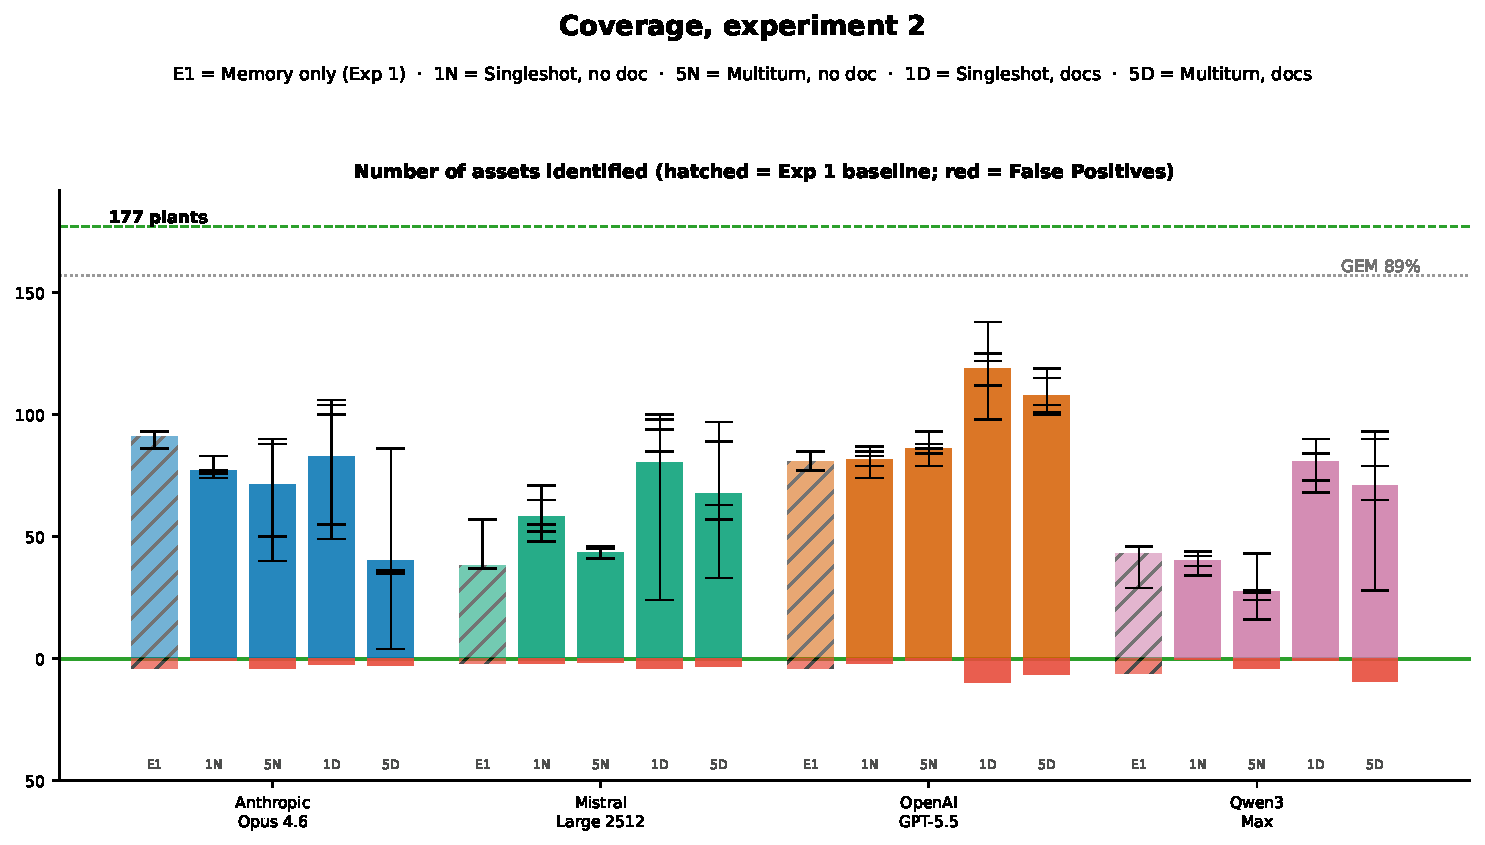
\includegraphics[width=\linewidth,keepaspectratio]{inputs/generated/fig_exp2_arms_coverage.pdf}
\caption{Expérience~2 (frontière SOTA)~: couverture (nombre d'actifs identifiés, en rouge les faux positifs), regroupée par agent. Les barres distinguent les deux bras enregistrés (sans documents) des deux conditions exploratoires (avec documents). Quatre agents, 5~répétitions par cellule.}
\label{fig:exp2-arms-comparison}
\end{figure}

\begin{figure}[h]
\centering
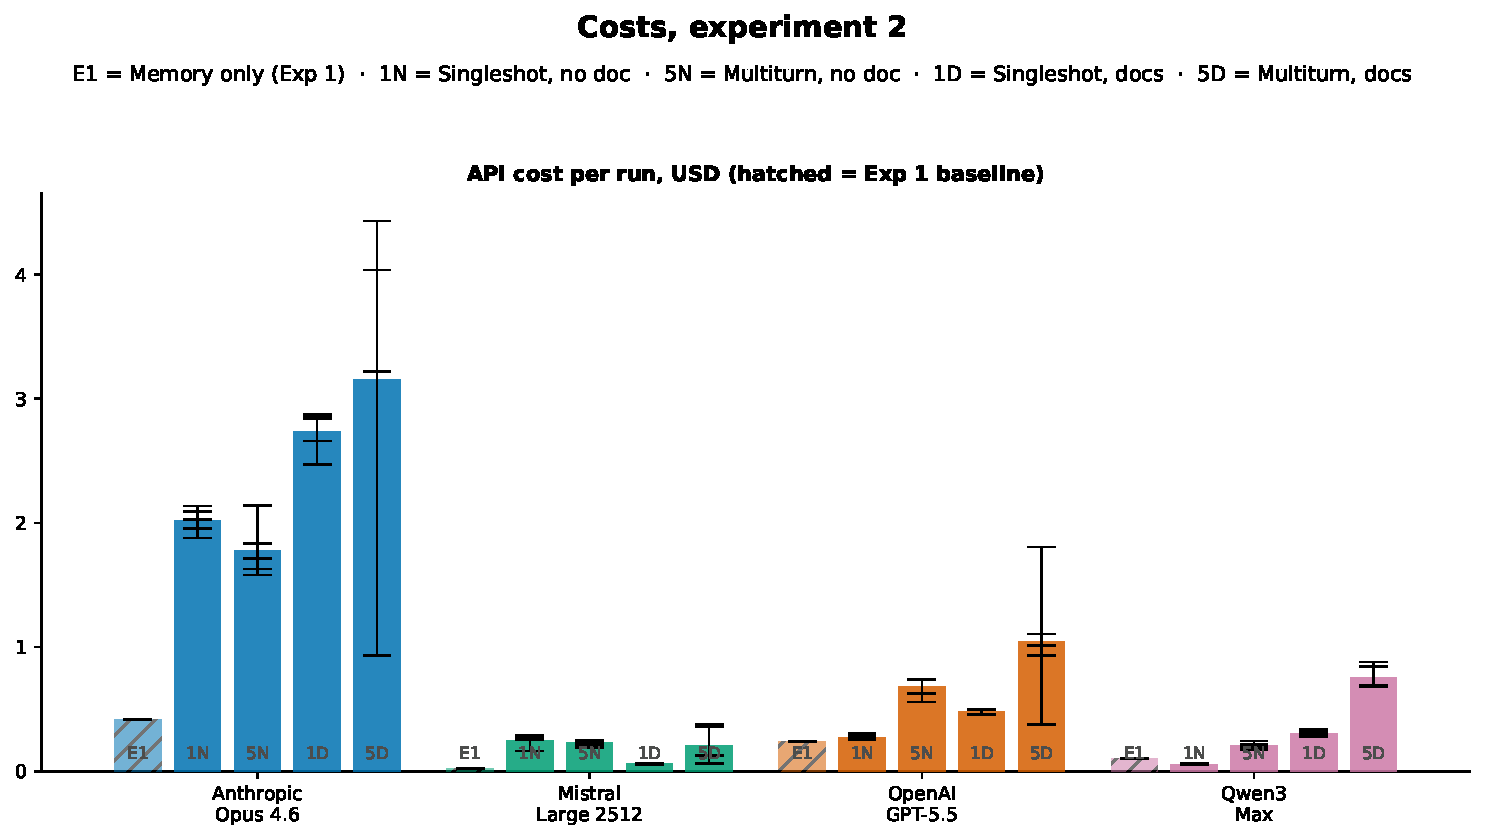
\includegraphics[width=\linewidth,keepaspectratio]{inputs/generated/fig_exp2_arms_cost.pdf}
\caption{Expérience~2 (frontière SOTA)~: coût API par exécution (USD), regroupé par agent. Le protocole multi-tours coûte sensiblement plus cher pour un gain de couverture limité. Quatre agents, 5~répétitions par cellule.}
\label{fig:exp2-arms-cost}
\end{figure}

\paragraph{Provenance des citations.} Le tableau~\ref{tab:exp2-bib-quality} agrège, par agent et par bras, la structure de citation des inventaires (lignes, taux de Source~1 et~2, part de sources primaires, taux de Notes, entrées bibliographiques), moyennée sur les seules exécutions parsables (\texttt{n\_rows}${>}0$), l'étendue figurant entre crochets. Ce tableau est purement descriptif et sert de socle de provenance aux audits ultérieurs (H5, conformité Wikipedia)~; son interprétation par agent est développée avec ces tests.

\InputIfFileExists{inputs/generated/tab_exp2_bib_quality}{}{}

\section{Résultats par hypothèse (H1--H6)}\label{sec:exp2-sota:hypotheses}

\subsection{H1~: F1 par ligne, bras optimisé vs naïf}
% TODO(0255)

\subsection{H2~: différences inter-agents sur les rangs de F1}
% TODO(0256)

\subsection{H3~: apport de la passe de vérification sur la traçabilité}
% TODO(0257)

\subsection{H4~: taux de bounce du bras naïf}
% TODO(0258)

\subsection{H5~: audit de conformité Wikipedia/Wikidata}
% TODO(0259)

\subsection{H6~: concordance évaluation croisée vs métriques mécaniques}
% gated on 0171 (Phase C cross-eval)
% TODO(0260)

\section{Synthèse}\label{sec:exp2-sota:synthese}
% TODO(0261)

\chapter{Documents sources et RAG}\label{chap:rag}

Ce chapitre traite de la découverte et préparation des documents sources, puis de leur rôle dans le pipeline de fusion incrémentale. Le Retrieval Augmented Generation (RAG) est ici un \emph{composant de récupération}~: il extrait des fragments depuis le corpus documentaire, fragments qui deviennent les entrées d'une fusion contrôlée produisant la table maître. Séparer l'extraction (RAG) de la fusion (pipeline) garantit la reproductibilité~: la fusion peut être déterministe même quand l'extraction ne l'est pas.

\section{Découverte et préparation des documents}

\subsection{Veille}

Les documents sont découverts par veille manuelle~: suivi de LinkedIn, abonnement à des newsletters spécialisées (Vietnam Energy Transition Update, Vietnam Infrastructure Updates), examen des sommaires de NangLuongVietnam.vn, et suivi des références bibliographiques. Les documents sont traduits si besoin, puis validés avant archivage~: le contenu doit avoir été vérifié par un expert pour entrer dans la base.

Il existe de nombreux services de bibliométrie académique et scientifique \citep{5WPNTHNM}, des bases traditionnelles (Web of Science, Scopus, Dimensions) aux outils AI récents (Elicit, Connected Papers, Scite). Au-delà des publications académiques, des acteurs comme AlphaSense ou Bloomberg proposent de l'intelligence économique. Notre optique est différente~: nous visons une connaissance ouverte du deep web, à l'échelle personnelle, accumulée sur le temps long, avec validation humaine avant ingestion dans la base.

\subsection{Indexation dans Zotero}

Les documents sont indexés dans Zotero \citep{9666795Z}, avec attention aux contraintes de multilinguisme et de normalisation des métadonnées. L'indexation automatique reste un défi~: plusieurs approches sont envisageables (métadonnées embarquées, archives DOI/ISBN, adaptateurs par source, LLM généraliste, ou modèles spécialisés comme GROBID).

\subsection{Conversion PDF vers Markdown}\label{sec:pdf-to-md}

La conversion des documents en Markdown améliore le traitement ultérieur par les LLM. Nous avons développé \emph{pdfOCR2md.py}, un script qui délègue l'OCR à un LLM et retourne du Markdown structuré. Selon les comparatifs \citep{ULQGRISS,RM4KCTEG}, faire reconnaître un PDF par un LLM généraliste est la solution la plus qualitative mais aussi la plus lente et onéreuse. Des solutions comme Docling, Marker, ou Mistral OCR offrent des compromis intéressants.

Nous avons comparé six backends de conversion sur un document de référence~: la Décision~1509/QĐ-BCT (173~pages, vietnamien scanné, tableaux complexes). Le tableau~\ref{tab:converter-benchmark} résume les résultats. Marker et Mistral~OCR~direct extraient chacun environ 170~tableaux avec les diacritiques du vietnamien préservés. MinerU~v3, avec accélération~GPU et le backend \emph{pipeline}, extrait 62~tableaux mais perd les diacritiques dans les cellules de tableaux (le texte courant est correct). GROBID extrait du texte de qualité mais aplatit la structure tabulaire. Les approches passant par un LLM intermédiaire (plugin Mistral~OCR, Cloudflare~AI) sont limitées par la fenêtre de sortie du modèle.

\begin{table}[htbp]
\centering
\caption{Comparaison de six backends de conversion PDF$\to$Markdown sur la Décision~1509 (173~pages). Colonnes~: tableaux détectés, lignes de données extraites, taille du Markdown, temps de traitement, et qualité des diacritiques du vietnamien. Les tirets (--) indiquent des backends ne produisant pas de structure tabulaire exploitable.}\label{tab:converter-benchmark}
\InputIfFileExists{inputs/generated/tab_converter_benchmark}{}{\textbf{[Table not generated]}}
\end{table}

\section{Stratégie RAG}

Le RAG joue le rôle de couche de récupération dans le pipeline de fusion~: il sélectionne les documents pertinents et en extrait les fragments tabulaires (les 15~tables Markdown du corpus, voir section~\ref{sec:pdf-to-md}) qui alimentent ensuite la fusion incrémentale. Le retrieval opère en deux étages~: trouver les documents pertinents parmi une base de milliers, puis extraire les passages intéressants (tables) parmi ces documents.

\subsection{Retrieval par LLM}

Exporter toute la bibliothèque Zotero (5.6~MB en JSON) et demander à un LLM de trouver les documents pertinents dépasse le context window de la plupart des modèles. Gemini-1.5-Pro-2M traite la requête pour un coût 350 fois supérieur à la version Flash, avec des résultats peu convaincants~: seuls 2 documents sur 20 contiennent des inventaires nationaux.

\subsection{Techniques de retrieval}

Les systèmes efficaces sont souvent hybrides~: scoring par LLM, recherche vectorielle par similarité sémantique, filtrage par mots-clés, ou encodage dans un réseau de connaissance. Pour cette étude de faisabilité, nous avons procédé par sélection manuelle raisonnée dans Zotero, en retenant les plans de développement du secteur électrique (PDP7, PDP7A, PDP8), des rapports d'implémentation, des newsletters et articles de presse, et trois jeux de données (Wikipedia, notre inventaire, Global Energy Monitor).

\subsection{Extraction des tables pertinentes}

Les pages d'annexes sont extraites des PDF et converties en Markdown (section~\ref{sec:pdf-to-md}), avec retouches manuelles. Au total, 15~fichiers Markdown contenant chacun une table, pour 138,6~kB soit 63~545 tokens~--- ces 15~fragments sériels constituent le corpus d'entrée de la fusion incrémentale (voir chapitre~\ref{chap:architecture}).

\section{Résultats du RAG}

On joint les 15 tables et leurs références bibliographiques au Prompt~2 (section~\ref{sec:methode}).

\InputIfFileExists{inputs/generated/tab_comparaison}{}{}

Les modèles de raisonnement sortis en janvier 2025 (Deepseek R1, o3-mini-high) donnent les meilleurs résultats avec relance. Les sources sont souvent citées de manière imprécise~: références globales au modèle plutôt que ligne par ligne, ou bien citations de documents plausibles mais non fournis.

Certaines centrales manquent systématiquement~: les anciennes retirées du service, celles antérieures au PDP7 (2011), les projets LNG non retenus par le PDP8, et les petites centrales captives industrielles. En ajoutant les rapports annuels de Vietnam Electricity, Claude~3.5~Sonnet atteint 101 centrales après relance.

\subsection{Évaluation par réconciliation}

On compare les résultats avec l'inventaire exhaustif compilé par nos soins à l'aide de \emph{reconcile.py}, un script de réconciliation par correspondance exacte et fuzzy matching.

Le seuil de similarité pour le fuzzy matching (par défaut~90 sur une échelle de 0 à~100) est un degré de liberté caché~: les modèles prolifiques (Gemini~Flash~Lite, Qwen~9B) dépendent davantage du matching flou que les modèles conservateurs (DeepSeek~V3.2). Pour vérifier que les classements ne sont pas un artefact du seuil choisi, nous effectuons un balayage post-hoc~: chaque paire matchée conserve son score de similarité brut, puis nous recalculons F1 pour des seuils allant de~75 à~95 sans relancer l'optimisation MILP. Sur les 44 modèles évalués, 35 inversions de classement apparaissent entre paires de modèles (principalement dans les conditions \emph{direct} et \emph{direct\_complete}), mais 17 modèles (39\,\%) forment un noyau stable dont le classement relatif est invariant sur tout l'intervalle de seuils. Les modèles les plus sensibles au seuil (pente F1 de $-0{,}012$ par unité) sont ceux du mode \emph{direct\_complete}, où le matching flou porte sur un plus grand nombre de paires. Pour les comparaisons rapportées dans les sections suivantes, nous privilégions les modèles du noyau stable et signalons les cas où une conclusion dépend du seuil choisi.

\begin{longtable}[]{@{}lllll@{}}
\caption{Performances de Claude selon différentes configurations~: nombre de centrales correctes, incorrectes et manquantes}\label{tab:performances}\\
\toprule
Configuration & Exactes & Approximatives & Incorrectes & Manquantes \\
\midrule
\endhead
\bottomrule
\endlastfoot
Claude (3.5 Sonnet) concise & 25 & 1 & 2 & 135 \\
Claude (normal) & 30 & 1 & 1 & 126 \\
Claude + relance & 53 & 2 & 7 & 98 \\
Claude + RAG & 43 & 6 & 1 & 105 \\
Claude + RAG + Relance & 61 & 12 & 9 & 72 \\
\end{longtable}

Les deux techniques (relance et RAG) sont complémentaires. Il manque encore beaucoup de lignes par rapport à notre référence, mais les centrales les plus importantes sont probablement incluses. Cette approche ne permet toutefois pas de remonter le pedigree complet des résultats.

\subsection{Qualité de la référence~: accord inter-annotateur}\label{sec:reconciliation}

L'inventaire de référence (\NumRefPlants~centrales) est la compilation d'un seul expert. Pour quantifier sa fiabilité, on le confronte à une seconde source indépendante~: le Global Energy Monitor (GEM, 153~centrales). La réconciliation par programmation linéaire (section~\ref{sec:methode}) produit 116~appariements~: 54~centrales de la référence experte sont absentes du GEM et 37~centrales du GEM sont absentes de la référence, de sorte que les deux sources se recoupent largement sans que l'une soit incluse dans l'autre.

L'accord sur les attributs est substantiel pour le combustible ($\kappa$ de Cohen = 0,601, accord brut 79\,\%), modéré pour la capacité (67\,\%) et faible pour le statut (47\,\%). Les désaccords de statut reflètent des ontologies différentes (GEM distingue \emph{pre-permit}, \emph{announced}, \emph{shelved} là où la référence experte utilise \emph{planned}, \emph{proposed}, \emph{cancelled}). Les désaccords de capacité proviennent d'agrégations différentes~: le GEM sépare parfois les phases d'un même site que la référence experte fusionne.

Pour mesurer l'effet de ces différences sur le classement des modèles, on réévalue les extractions de l'Expérience~1 contre les deux références. Le rang de Spearman entre les F1 médians obtenus avec la référence experte et avec le GEM est $\rho = 0{,}668$ ($p = 0{,}007$, $n = 15$ modèles)~: le classement des modèles est positivement corrélé entre les deux références, mais il n'est pas insensible au choix de celle-ci.

\InputIfFileExists{inputs/generated/tab_reconciliation}{}{}

\section{Expérience 3~: RAG wholesale à l'échelle}\label{sec:rag}

On étend l'évaluation RAG à 17 modèles couvrant deux familles (Qwen~3.5, Gemma~4) et trois tiers d'infrastructure (edge 2--4B, station de travail 9--35B, cloud 122B+), chacun interrogé 3 fois dans les mêmes conditions~: corpus RAG wholesale de 18 documents (37\,283 tokens), même prompt, pas de relance. L'inventaire de référence compte \NumRefPlants{} centrales thermiques.

\InputIfFileExists{inputs/generated/tab_per_run}{}{}

Les résultats révèlent deux régimes d'erreur distincts. Quatre modèles (DeepSeek, GPT, Mistral~Large, Mistral~Small) sont \emph{limités par la troncature}~: chaque centrale retournée est correcte (précision 100\,\%, zéro hallucination), mais la réponse est coupée avant d'être complète. Le nombre de centrales varie fortement entre les runs (de 4 à 141), ce qui indique une instabilité dans la longueur de sortie plutôt qu'un manque de connaissance. Le meilleur résultat individuel est Qwen~3.5-122B (117 centrales, F1 = 71,8\,\%).

Gemini~2.5~Flash~Lite présente le régime inverse~: un rappel élevé (jusqu'à 138/\NumRefPlants{} centrales thermiques trouvées), mais il ajoute un nombre variable de centrales non thermiques (hydroélectriques, éoliennes, nucléaires)~--- de 88 dans le meilleur cas à 505 dans le pire.

\subsection{Agrégation multi-runs (self-consistency)}

Puisque chaque modèle est interrogé 3 fois, on peut agréger les résultats par vote majoritaire (plante retenue si présente dans 2+ runs) ou par union (plante retenue si présente dans au moins 1 run).

\InputIfFileExists{inputs/generated/tab_self_consistency}{}{}

Le vote majoritaire est inadapté aux modèles limités par la troncature~: il prend l'intersection de sous-ensembles déjà incomplets, réduisant davantage le rappel. En revanche, il profite à Gemini car l'intersection filtre les hallucinations non thermiques.

Le vote par union bénéficie aux modèles tronqués~: les 3 runs de DeepSeek couvrent collectivement davantage de centrales que le meilleur run individuel (83 centrales). Le choix de la stratégie d'agrégation dépend donc du mode de défaillance du modèle~: union pour la troncature, majorité pour la surgénération.

\subsection{Requête RAG par type de combustible}\label{sec:rag_per_fuel}

La troncature étant le principal facteur limitant, on teste une stratégie de décomposition~: au lieu d'une seule requête demandant toutes les centrales thermiques, on envoie 3 sous-requêtes par type de combustible (charbon, gaz/GNL, pétrole/autres), chacune avec le même corpus RAG. Les 3 réponses CSV sont extraites puis fusionnées avec dédoublonnage par nom.

\InputIfFileExists{inputs/generated/tab_decomposition}{}{}

La décomposition améliore le rappel~: le meilleur run atteint 154 centrales sur \NumRefPlants{}, contre un maximum de 117 en requête unique. L'effet net sur le F1 dépend du modèle~: fortement positif pour les modèles qui étaient limités par la troncature, mais variable pour les modèles déjà performants en requête unique.

Le meilleur résultat absolu est DeepSeek~V3.2 décomposé~: sur $n=4$ réplicats, F1 moyen = 68,6\,\% [60,7--74,8\,\%, IC 95\,\%], meilleur run 76,5\,\%, pour un coût de 0,06~\$ par run. La variance élevée (écart de 19 points entre runs) reflète la sensibilité de la décomposition au bruit d'échantillonnage du LLM.

Le principal inconvénient est massif et dépasse largement la simple fuite inter-catégories~: la décomposition introduit des hallucinations systématiques là où la requête unique n'en produisait aucune. Pour une même base documentaire et un même jeu de référence, le taux de faux positifs (entrées du système absentes de la référence) passe de 0\,\% à 40--52\,\% chez GPT-5.4, et de 0\,\% à 19--29\,\% chez Mistral~Small (tableau~\ref{tab:decomposition-fp}). Les trois modèles stables en RAG de base (GPT-5.4, DeepSeek, Mistral~Large) se comportent tous ainsi~: zéro hallucination en requête unique, plusieurs dizaines en décomposition.

\begin{table}[htbp]
\centering
\caption{Taux de faux positifs (lignes système absentes de la référence), RAG de base vs décomposé, 3 runs par modèle.}\label{tab:decomposition-fp}
\begin{tabular}{@{}lll@{}}
\toprule
Modèle & Requête unique & Décomposé \\
\midrule
GPT-5.4             & 0 / 0 / 0\,\%   & 45 / 40 / 52\,\% \\
DeepSeek V3.2       & 0 / 0 / 0\,\%   & 20 / --- / 2\,\% \\
Mistral Large       & 0 / 0 / 0\,\%   & 7 / 25 / 10\,\% \\
Mistral Small       & 0 / 0 / 0\,\%   & 29 / 0 / 19\,\% \\
Gemini 2.5 Flash Lite & 59 / 6 / 75\,\% & 40 / 64 / 0\,\% \\
\bottomrule
\end{tabular}
\end{table}

L'inspection des lignes fabriquées révèle trois motifs. D'abord, un \textbf{fractionnement en unités}~: les centrales agrégées sont décomposées en lignes par tranche (\textit{An Khanh 1 Unit 1}, \textit{Unit 2}, 50~MW chacune, au lieu de l'agrégat \textit{An Khánh~1} à 116~MW de la référence), systématique chez GPT-5.4 sur \textit{Vung~Ang~1}, \textit{Duyen~Hai~1}, \textit{Thai~Binh~1}. Ensuite, des \textbf{fuites de combustible}~: \textit{O~Mon~1~Unit~2}, une centrale à gaz, apparaît dans la sortie charbon avec fuel \textit{unknown}. Enfin, un cas extrême de défaillance de sortie structurée~: la ligne 181 de la réconciliation contient un <<~nom de centrale~>> littéralement égal à \texttt{"Lai~Chau~is~hydro"}, capacité 0~MW, fuel \texttt{coal}. Le modèle a écrit de la prose dans le champ nom, et l'extracteur l'a accepté.

L'analyse du code (\texttt{src/aedist/query\_per\_fuel.py} lignes~55--77) désigne une cause~: les trois sous-prompts exigent explicitement du modèle qu'il dépasse le corpus. La consigne \textit{<<~Be absolutely exhaustive --- include operational, under construction, planned, proposed, and cancelled plants.~>>} est présente dans chaque sous-requête, alors que le prompt de base (\texttt{experiments/prompts/prompt\_structured.txt}) est laconique et ne demande aucune exhaustivité. En requête unique, le modèle reste à l'intérieur du corpus. Pour satisfaire l'injonction <<~soyez exhaustif, incluez les centrales annulées~>>, le modèle n'a qu'une issue~: se replier sur sa mémoire paramétrique, fractionner les agrégats qu'il a mémorisés et fabriquer les noms dont il se souvient vaguement. La \textbf{leçon méthodologique} est générale et mérite d'être isolée~: dans un cadre RAG, toute consigne d'exhaustivité qui excède le périmètre du corpus transforme la mémoire paramétrique en source de secours, et donc l'absence documentaire en hallucination. La réparation — supprimer la consigne d'exhaustivité et ajouter une clause d'ancrage (\textit{<<~based only on the provided documents~>>}) — est testée dans le ticket~0068.

La correction est évaluée sur un second lot de runs (tableau~\ref{tab:decomposition-fix}). Les taux y sont calculés avec le scoreur courant et la référence v2~: les lignes appariées par nom mais à capacité discordante (\emph{Mismatched}) comptent désormais comme faux positifs, alors qu'une version antérieure du scoreur les créditait à tort comme reconnaissances. Sous cette mesure corrigée, l'effet de la clause d'ancrage est plus modeste qu'initialement rapporté~: le FP moyen va de 24,0 à 50,9\,\% dans le bras initial contre 14,0 à 36,6\,\% dans le bras corrigé, et pour DeepSeek~V3.2, seul modèle présent dans les deux bras, le taux reste stable (24,0\,\% contre 25,0\,\%). L'inspection des lignes de réconciliation montre qu'une grande part des FP résiduels sont des actifs hors du périmètre de la référence thermique (hydraulique d'importation, solaire, nucléaire, lignes agrégées), un fond commun aux deux bras que la clause d'ancrage ne vise pas. La correction réduit les fabrications pures sans éliminer ce fond~: le meilleur modèle du bras corrigé (Gemini~3~Flash, 14,0\,\%) reste toutefois bien en deçà des pires taux du bras initial.

\InputIfFileExists{inputs/generated/tab_decomposition_fix}{}{}

\subsection{Extraction RAG citée}\label{sec:rag_cited}

Le pipeline RAG peut-il fournir non seulement des données mais aussi leur provenance ligne par ligne~? On ajoute au prompt deux colonnes de citation (\texttt{source\_1}, \texttt{source\_2}) et une colonne de notes, demandant pour chaque centrale une ou deux sources primaires (décisions gouvernementales, rapports annuels, relevés du régulateur). L'expérience porte sur Claude~Opus~4.6 en mode RAG wholesale (même corpus de 18~documents), avec 3~runs indépendants.

Les trois runs retournent respectivement 120, 115 et 102~centrales (F1 = 0,85 ; 0,83 ; 0,77), toutes avec précision 100\,\% (zéro faux positif). Les citations sont spécifiques~: numéro de page du rapport annuel EVN, annexe du PDP, numéro de décision (\emph{Quyết định}). Sur les 337~lignes cumulées, 77\,\% des citations renvoient à des sources primaires et aucune source fabriquée n'a été identifiée lors d'une vérification manuelle. La variance entre runs (18~centrales d'écart) provient de la troncature de sortie, non d'une dégradation de la qualité des citations. Le coût moyen est de 0,76\,\$ par run (87\,k~tokens d'entrée, 13\,k de sortie).

Ce résultat montre que le mode RAG wholesale, combiné à un prompt de citation, produit des données traçables sans perte de précision. La limite est le rappel~: même le meilleur run ne retrouve que 64\,\% des \NumRefPlants{}~centrales de référence. La combinaison des deux approches --- décomposition pour le rappel, citations pour la traçabilité --- est un axe de travail futur.

\subsection{Cohérence interne}

Au-delà de la comparaison avec la référence, la \textbf{cohérence interne} des extractions est un indicateur de qualité indépendant~: les données extraites sont-elles auto-cohérentes~? Pour chaque extraction, trois niveaux de vérification sont appliqués automatiquement~: (1)~au niveau de la ligne (capacité positive, combustible et statut connus, province reconnue), (2)~entre lignes (détection de doublons), et (3)~au niveau agrégé (totaux de contrôle). Le taux de cohérence est la proportion de lignes sans problème détecté (tableau~\ref{tab:coherence}).

\InputIfFileExists{inputs/generated/tab_coherence}{}{}

% Verification methods — redesigned for 3-tier audit-verified verification
% Included from report.tex, inside section "Exp 3: RAG wholesale" after decomposition
%
% Replaces the 5-mode post-hoc protocol (unverified / tool / self / cross / web
% + rubric 0-4). The negative result motivating the replacement is ticket interne
% 0059 (PR #246): 0–10% inter-verifier agreement even after bugfix.
% Current design: front-loaded HITL source triage + 3-tier deterministic chain.
% See also slides/slides.tex §"Fiabilité" for the full framing.

\subsection{Vérification des sources}\label{sec:verification}

Les expériences précédentes mesurent la \emph{couverture} de l'extraction~:
combien de centrales le modèle trouve-t-il~? Mais pour un modélisateur de
systèmes énergétiques, la couverture ne suffit pas~: chaque donnée intégrée
dans un scénario doit être traçable jusqu'à un document source
(section~\ref{chap:conclusion}).

\subsubsection{Pourquoi la vérification LLM \emph{post-hoc} échoue}\label{sec:verif-postHoc}

Une première approche préenregistrée demandait à des panels de modèles de
vérifier chaque ligne extraite en citant les sources qui l'étayent, puis
d'agréger les scores par vote majoritaire. Le ticket interne~0059 (PR~\#246)
établit que ce protocole est une impasse~: l'accord inter-vérificateurs
atteint 0~à~10\,\%, même après correction d'un bogue d'appariement. La
cause profonde est structurelle~: la rubrique 0--4 demande aux modèles de
rappeler des citations depuis leur mémoire paramétrique, produisant des
opinions et non de la provenance. Un modèle peut confirmer avec confiance une
fabrication qu'il a lui-même produite. L'indépendance statistique entre
vérificateurs, supposée par l'architecture multi-agents, est minée par les
biais d'entraînement communs. La vérification \emph{post-hoc} par LLM ne
s'améliore pas avec davantage de vérificateurs~: elle converge vers du bruit
inter-modèles.

\subsubsection{Justification du \emph{front-loading}}\label{sec:verif-frontload}

Le rendement épistémique de la vérification est inversement proportionnel au
moment où elle intervient. Une intervention humaine en amont --- le triage
des sources avant toute extraction --- est l'acte de contrôle qualité le plus
levier avec le coût le plus bas. L'opérateur valide les éditeurs, pas les
cellules~: les décisions gouvernementales (\emph{Quyết định}), les rapports
annuels d'EVN et les données du régulateur sont classées sources primaires~;
les newsletters économiques et les compilations secondaires sont écartées.
Ce filtre éditorial élimine une large fraction des fabrications potentielles
avant même le premier appel LLM. Les sources validées sont ensuite
téléchargées, converties en Markdown, indexées et archivées. L'extraction RAG
opère sur ce corpus vérifié, actif par actif. Le résultat est un jeu de
données dont chaque cellule est traçable jusqu'à un document source~--- non
pas des données correctes, mais des données \emph{corrigeables}~: quand un
relecteur trouve une erreur, le pipeline indique quelle source était erronée
et quoi corriger.

\subsubsection{Vérification déterministe à trois niveaux}\label{sec:verif-tiers}

La vérification automatisée suit une chaîne à trois niveaux, par ordre
croissant de coût et de subjectivité~:

\begin{description}
\item[Niveau~1 --- correspondance de chaînes.]
  Chaque cellule extraite est confrontée déterministiquement à la table
  source~: appariement flou du nom de fichier et du nom de la centrale, puis
  recherche de la valeur numérique dans le document correspondant. Le résultat
  est binaire~: \emph{ancré} (la valeur est retrouvée dans la source citée)
  ou \emph{échec}. Sur le corpus thermique vietnamien avec extraction sourcée
  (3~runs Opus), le taux d'ancrage médian est de~98\,\%~; la traçabilité
  complète (valeur retrouvée et centrale identifiée dans le document) atteint
  80\,\% en médiane. La baseline sans sources affiche~0\,\% dans les deux
  métriques (tableau~\ref{tab:source-grounding}).

\item[Niveau~2 --- adjudication LLM.]
  Quand le niveau~1 échoue, un LLM reçoit la cellule, la source citée, et la
  question~: \emph{la valeur est-elle compatible avec ce document~?} Sa
  réponse est une règle candidate (alias, unité, terme local ou synonyme
  d'attribut) qui explique l'écart. Cette règle n'est pas appliquée
  automatiquement~; elle est transmise au niveau~3 pour ratification.

\item[Niveau~3 --- mémoire ratifiée par HITL.]
  Un opérateur humain examine la règle candidate, sa justification et la
  cellule d'évidence. S'il ratifie, la règle est écrite dans la mémoire du
  système (un fichier \texttt{audit.jsonl} versionné sous git). Les runs
  ultérieurs l'appliquent au niveau~1, réduisant le taux d'escalade au
  niveau~2 à chaque itération.
\end{description}

\noindent Ce design place le déterminisme en premier et n'engage le LLM qu'en
recours. L'humain ratifie chaque règle une fois, pas chaque cellule à chaque
fois~: le coût de supervision décroît à mesure que la mémoire s'enrichit.

\subsubsection{Quatre catégories de règles}\label{sec:verif-rules}

Les règles en mémoire appartiennent à quatre catégories, chacune encodant un
type distinct de divergence entre la valeur extraite et la valeur dans la
source~:

\begin{description}
\item[Alias.]
  Identité d'entité~: deux noms désignent la même centrale.
  Exemple~: \texttt{«~VT1~»} $\equiv$ \texttt{«~Vinh Tan~1~»} dans le
  corpus PDP8. Une règle d'alias permet à l'appariement du niveau~1
  de résoudre la correspondance sans escalade.

\item[Unité/format.]
  Forme de valeur~: la cellule extraite et la source expriment la même
  quantité dans des formats différents.
  Exemple~: \texttt{«~1~200~MW~»} $\to$ \texttt{1200.0~MWe} (espace de
  millier, suffixe d'unité, virgule décimale). La règle normalise avant
  comparaison.

\item[Terme source-local.]
  Vocabulaire spécifique au corpus~: un terme ou une abréviation propre à un
  document source particulier.
  Exemple~: \texttt{«~Nhóm~»} dans le PDP8 désigne un groupement de
  tranches (\emph{Group}) que le modèle peut retranscrire autrement.

\item[Synonyme d'attribut.]
  Correspondance colonne--schéma~: le modèle utilise une désignation
  d'attribut différente de celle du schéma cible.
  Exemple~: \texttt{«~en construction~»} $\to$ statut \texttt{constructing}
  dans la table de référence.
\end{description}

La mémoire croît de façon monotone, commitée dans git et révisable via diff.
Chaque règle porte un raisonnement, des cas limites et des preuves~: un
carnet de terrain pour le prochain statisticien, et non un script de
substitution mécanique.

\subsubsection{Piste d'audit}\label{sec:verif-audit}

Chaque règle en mémoire est accompagnée de cinq champs d'audit, qui
permettent à un second témoin de retracer et de contester n'importe quelle
décision~:

\begin{enumerate}
\item \texttt{source\_llm\_suggestion} --- le modèle et le prompt qui ont
  proposé la règle candidate (niveau~2) ;
\item \texttt{ratifying\_human} --- l'identifiant de l'opérateur qui a
  ratifié (niveau~3) ;
\item \texttt{timestamp} --- horodatage UTC de la ratification ;
\item \texttt{evidence\_cell} --- la cellule et le document source qui ont
  déclenché l'escalade au niveau~2 ;
\item \texttt{witness} --- résultat de la vérification par un second
  opérateur (échantillonnage).
\end{enumerate}

\noindent L'ensemble est committé dans git~; toute modification future est
visible dans l'historique de diff.

Les métriques de suivi de la mémoire sont~: le \emph{taux d'escalade par
étape de fusion} (\texttt{escalation\_rate\_per\_step}), la \emph{croissance
du nombre de règles} par catégorie (\texttt{rule\_count\_growth}), et le
\emph{taux d'acceptation des ratifications}
(\texttt{ratification\_acceptance\_rate}). Un taux d'escalade décroissant
confirme que la mémoire apprend~; un taux d'acceptation faible signale une
dérive du niveau~2 ou une frontière de catégorie mal calibrée.


% plan_verification_multi and results_verification_multi were the
% preregistered 5-mode post-hoc LLM protocol (ticket 0054 / 0059).
% Superseded by the 3-tier deterministic design (tickets 0097 / 0099).
% Files kept as historical artifacts; no longer rendered in this report.

\section{Pièges méthodologiques}\label{sec:pitfalls}

% TODO: deux paragraphes + deux figures (à rédiger après les slides)
%
% \subsection{Décomposition par combustible}
% Paragraphe : la décomposition résout la troncature mais introduit des
% artefacts (centrales hydroélectriques dans la catégorie "autres combustibles",
% double-comptage aux frontières des catégories). Figure : taux de faux positifs
% par catégorie avant/après déduplication.
%
% \subsection{Union de runs}
% Paragraphe : l'union-of-runs exploite la variance stochastique pour gonfler
% le rappel — les runs non-déterministes produisent des listes différentes,
% et leur union dépasse ce qu'un run unique contrôlé peut atteindre. À T=0
% les runs sont identiques et l'union n'apporte rien. Présenter ce chiffre comme
% résultat revient à optimiser sur le bruit. Figure : F1 union vs F1 médian par
% modèle, montrant que l'écart disparaît à T=0.

\section{Discussion}

\subsection{Triage des faux négatifs}\label{sec:fn-triage}

Que recouvre exactement le déficit de rappel~? Les centrales de référence non retrouvées (faux négatifs) sont comptées en agrégat, mais ce chiffre confond des causes distinctes~: limite du comparateur, trou dans la référence, désaccord de périmètre, et échec de rappel véritable. Pour le quantifier, les 40~faux négatifs du meilleur run RAG (GPT-5.5, run~4) ont été triés un par un, en confrontant chaque centrale manquée à la sortie du modèle et au contenu du corpus fourni (tableau~\ref{tab:exp3-fn-triage}). La feuille de triage, avec justification ligne par ligne, est versionnée (\texttt{experiments/derived/exp3\_fn\_triage.csv}).

\InputIfFileExists{inputs/generated/tab_exp3_fn_triage}{}{}

Le constat principal~: moins de la moitié des faux négatifs (18 sur 40, soit 45\,\%) sont des échecs de rappel véritables --- c'est le signal de référence du banc d'essai. Le reste est imputable à notre dispositif d'évaluation. Le \textbf{comparateur} explique 16~cas (40\,\%)~: le modèle a bien produit la centrale, mais sous une granularité différente (ligne agrégée de site face aux tranches de la référence, comme \textit{Nhơn Trạch 3~et~4} en une seule ligne de 1\,624~MW~; extension \textit{MR} fondue dans l'unité de base~; complexe industriel décliné par unité de 150~MW), sous un alias (\textit{Long Sơn hóa dầu} pour \textit{Long Son Chemical}), ou à travers un changement d'identité du projet (charbon annulé devenu LNG à \textit{Quảng Trạch~II}). La catégorie \textbf{liste} (centrale valide absente de la référence) est vide --- la référence avait déjà été auditée, et ce zéro en est la trace. La catégorie \textbf{définition} compte 6~cas (15\,\%)~: tous des lignes de la référence en-deçà du plancher d'entité que le prompt articule (statut <<~exploring~>> antérieur à \textit{Announced}, agrégats multi-provinces sans site, capacité nulle).

Le résidu lui-même se décompose. Sur les 18~échecs de rappel véritables, 11 portent sur des centrales dont la preuve figurait dans les documents fournis (défaut d'ancrage~: le modèle avait l'évidence sous les yeux, typiquement dans les tableaux de sites potentiels de l'étude E-542, et ne l'a pas restituée), 6 sur des centrales absentes du corpus (échec de la mémoire paramétrique seule, par exemple les projets J-Power de Dung Quat), et 1 cas de rétention de provenance~: le modèle connaît le projet LNG de Hải Phòng ajouté par le PDP8 révisé de 2025, le dit dans sa narration, mais refuse de l'inscrire faute de source consultable --- un respect de la consigne, non un échec de rappel. Pour le banc d'essai, la conséquence est directe~: le déficit de rappel apparent surestime d'un facteur deux l'échec du modèle, et la première marge de progression est le comparateur (liaison d'entités), pas le modèle.

Les progrès dans la technologie RAG sont rapides \citep{UEIVYTV4,SQX6VZRP}. L'écosystème comprend des solutions RAG-as-a-Service (GraphLit, SciPhi/R2R) et de nombreuses piles libres (Kotaemon, RagFlow, Verba, Khoj, AnythingLLM). Le système Deep Research d'OpenAI \citep{Y6A39QJJ} est capable de trouver et analyser des sources en ligne pour produire un rapport structuré. L'analyse de documents joints est devenue une fonctionnalité standard des interfaces de chat.

\chapter{Graphes de connaissances}\label{chap:kg}

Pour produire des statistiques rigoureusement sourcées et traçables, on s'intéresse à l'\textbf{extraction d'information} structurée \citep{MZNGHBPG,D2S7WQT2,P7LFRX4U}. Cette approche repose sur trois piliers~: la résolution d'entités (associer les différentes mentions d'une même centrale à une entité canonique), la traçabilité des sources (lier chaque assertion à sa provenance conformément aux normes W3C PROV \citep{LXQUK658}), et la fusion de données pour résoudre les conflits entre sources divergentes \citep{RI2MXYYS}.

\section{Ontologie et modèle de données}

Un modèle de données reste indispensable pour structurer le graphe. L'\textbf{Open Energy Ontology} (OEO)\footnote{\url{https://openenergyplatform.org/ontology/}} définit un modèle sémantique ouvert pour le domaine de l'énergie, avec 15 types de centrale électrique \citep{G49STI5L}. Elle fournit un vocabulaire commun pour harmoniser les données entre systèmes, tout en restant extensible aux spécificités régionales. D'autres ontologies comme Schema.org, Dublin Core ou DBpedia offrent des dénominateurs communs moins spécialisés.

\section{Interrogation des graphes globaux}

Plusieurs graphes de connaissance globaux ont été interrogés sur notre cas d'étude. Les exemples historiques incluent Cyc (1984), DBpedia (2007), le Google Knowledge Graph (2012) et Wikidata (2012). Les résultats varient considérablement~:

\begin{description}
\item[OpenStreetMap] Une requête Overpass retourne \textbf{42 centrales} existantes avec coordonnées géographiques et périmètres. C'est la source la plus riche pour les centrales en service, avec des informations sourcées (Wikidata, GEM). En revanche, OSM ne contient pas les projets planifiés.
\item[Diffbot] Retourne \textbf{54 résultats} pour les SPV de centrales thermiques au Vietnam, avec adresse, employés et revenus. Les informations ne sont pas sourcées \citep{U6PVXXZP}.
\item[Wikidata] Une requête SPARQL retourne \textbf{20 centrales} avec capacité pour 9 d'entre elles. La classification des types est peu claire, la liste incomplète, les sources lacunaires.
\item[DBpedia] Retourne entre 4 et 20 centrales selon la formulation de la requête, avec de nombreux doublons liés aux versions linguistiques multiples de Wikipedia et aux jointures SPARQL. La disponibilité du service est intermittente.
\end{description}

Ces résultats montrent que les graphes globaux sont complémentaires mais aucun n'est suffisant seul. La fiabilité et la disponibilité des points d'accès SPARQL posent un défi supplémentaire.

\section{Fusion graphes de connaissances et LLM}

Les graphes de connaissance (approche symbolique) et les LLM (approche statistique) sont complémentaires~: les premiers offrent une structure explicite et vérifiable, les seconds excellent en génération et compréhension contextuelle. La fusion de ces approches est un axe de recherche très actif \citep{8U2Q2H5E,8XXG9DKM,HFQGE3UK,MNQFVIVR,D7EXWP53,THNWVF3G,E42E7D4X,AZ5B27ML,TDG5RFPC,MZNGHBPG}.

Le framework \textbf{KAG} (Knowledge Augmented Generation) \citep{74SRYH2Q} illustre bien cette direction. Il introduit une représentation des connaissances adaptée aux LLM, une indexation croisée entre graphe et texte assurant la traçabilité, un alignement sémantique pour harmoniser les entités, et un moteur hybride décomposant les requêtes complexes en sous-questions logiques. Ces idées sont directement pertinentes pour produire des statistiques énergétiques traçables.

L'approche G-T2KG \citep{A8YXRKGQ} propose une construction de graphes indépendante du domaine, combinant OpenIE avec validation par LLM, démontrant un bon rappel et une bonne précision sur des domaines variés.

\section{Synthèse}

Il n'existe pas aujourd'hui de solution automatique complète pour extraire la connaissance structurée d'une collection de documents. Cependant, une approche avec validation humaine est envisageable~: comprendre la tâche en termes d'entités OEO, sélectionner les documents et passages pertinents, construire un graphe par document, identifier et compiler les assertions sur chaque centrale, fusionner les graphes pour déterminer les valeurs finales, et vérifier le résultat. Ce processus garantit que chaque donnée est traçable et accompagnée de métadonnées explicites.

\chapter{Systèmes agentiques}\label{chap:agents}

Les systèmes multi-agents permettent de décomposer la tâche complexe du suivi de la transition énergétique en modules spécialisés coordonnés par un orchestrateur \citep{W45HUZN5,MW2ME5P3}. Pour un système d'observation, on distingue plusieurs rôles~:

\begin{description}
\item[Agent Veilleur] Surveille les sources et classifie les nouveaux contenus.
\item[Agent Curateur] Gère l'indexation, l'ingestion vectorielle et la construction du graphe de connaissances.
\item[Agent Analyste] Extrait les entités et relations, fusionne les informations en tenant compte de la fiabilité des sources.
\item[Agent Rédacteur] Synthétise les résultats en rapports structurés avec vérification des sources.
\end{description}

L'écosystème des frameworks agentiques est en pleine expansion~: LangGraph, LlamaIndex, PydanticAI, Microsoft Semantic Kernel, Agno, et d'autres\footnote{OpenManus, HuggingFace Smolagent, Letta, Langroid, Swarms. Le protocole MCP standardise la communication.} \citep{ZF27JTIS,CVBHDNL3,LKNBDMMK}. Cependant, les systèmes combinant agents, RAG et graphes de connaissances restent à la frontière de l'ingénierie.

\section{Tests de systèmes existants}

\textbf{R2R} (SciPhi) \citep{S95D9L3Y} combine ingestion multimodale, recherche hybride et construction automatique de graphes de connaissances. Testé sur nos 18 tables en Markdown, le système construit un graphe d'environ 270 entités et 290 relations (version Docker locale), mais sans ontologie claire. Le mode RAG Agent retourne 29 centrales, le mode Question and Answer 43. L'interface entre le graphe et le RAG reste préliminaire.

\textbf{TrustGraph} propose une infrastructure modulaire combinant graphes de connaissances et bases vectorielles pour déployer des agents AI. La plateforme se positionne davantage comme une solution entreprise.

Ces résultats confirment que l'écosystème est encore immature pour notre cas d'usage~: la construction automatique de graphes sans ontologie produit des résultats incomplets, et l'intégration RAG-graphe n'est pas encore opérationnelle dans les outils testés.

\chapter{Architecture proposée}\label{chap:architecture}

\section{Pipeline comme fusion d'information}

L'architecture AEDIST v0 est organisée autour d'une primitive unique~:

\begin{center}
$\mathrm{master} + \mathrm{fragment} \longrightarrow \mathrm{master}'$
\end{center}

Un fragment est une pièce d'information extraite d'un document source. Trois types se distinguent par leur mécanique d'extraction et de fusion. Les \textbf{fragments sériels} sont des tables complètes (annexes des PDP, rapports EVN)~; leur intégration requiert un alignement de schéma et une liaison d'enregistrements~--- ils définissent le squelette de la table maître. Les \textbf{fragments multi-scalaires} sont des listes en prose (<<~la province X comprend les projets A, B, C~>>)~; leur fusion vérifie l'existence d'entités et confirme ou ajoute des lignes. Les \textbf{fragments scalaires} sont des faits isolés (<<~Vinh Tan~1 mise en service 2018~>>)~; leur fusion met à jour un attribut d'une entité déjà connue. Le prototype v0 traite les fragments sériels~: les 15~tables Markdown du corpus (section~\ref{sec:pdf-to-md}), chacune issue d'un document officiel vietnamien. Les types multi-scalaires et scalaires sont différés.

Séparer l'extraction (RAG, chapitre~\ref{chap:rag}) de la fusion garantit la reproductibilité~: la fusion peut être déterministe même quand l'extraction ne l'est pas. Chaque étape produit un diff inspectable. Le coût croît en $N$~sources, pas en $N \times S$ (fragments $\times$ sources). L'échec est localisé à une étape.

\section{Fondements décisionnels : fusion sous information imprécise}\label{sec:imprecise}

La primitive $\mathrm{master}+\mathrm{fragment}\rightarrow\mathrm{master}'$ instancie un problème plus ancien que les LLM~: fusionner des informations issues de sources de fiabilité inégale, en vue d'une décision, sans disposer de la vérité-terrain. Le cadre théorique adapté est celui des \emph{probabilités imprécises}, où l'information n'est pas représentée par une loi de probabilité unique mais par un ensemble convexe de lois admissibles (ensemble crédal), et où une masse de croyance peut être affectée à l'ensemble vide, $m(\emptyset)$, pour représenter les états du monde non décrits \citep{HaDuong2005}. Trois enseignements de ce cadre éclairent la fusion telle qu'elle est implémentée ici et tracent ses versions ultérieures.

\emph{Les sources corrélées créent une fausse précision.} La théorie distingue la conjonction \emph{non interactive}, qui suppose les sources indépendantes et dont le recoupement resserre légitimement les bornes, de la conjonction \emph{prudente} (idempotente), appropriée lorsque les sources «~se connaissent et partagent les mêmes données~» \citep{HaDuong2005}. Or nos sources ne sont pas indépendantes~: les LLM interrogés ont vraisemblablement été entraînés sur les mêmes graphes ouverts (OpenStreetMap, Wikipedia) qui servent par ailleurs de référence, de sorte qu'un accord entre un modèle et ces graphes relève souvent de la restitution mémorisée, non d'une corroboration indépendante. Compter de tels accords comme des confirmations distinctes gonflerait artificiellement la confiance. Le journal de fusion enregistre les confirmations dans une piste d'audit séparée du sidecar précisément pour ne pas les confondre avec des sources indépendantes au moment d'arbitrer une cellule~; pondérer la fusion par le \emph{nombre de sources effectivement indépendantes} reste une question ouverte, déjà posée dans ce cadre \citep{HaDuong2005}.

\emph{L'incomplétude se mesure et se distingue du conflit.} Dans le modèle des croyances transférables, $m(\emptyset)$ admet deux lectures~: un degré de contradiction entre sources, et un degré de \emph{monde ouvert}, la masse de croyance qui n'est attachée à aucun état décrit \citep{HaDuong2005}. AEDIST sépare délibérément ces deux quantités. Le désaccord entre extractions relève du contrôle de cohérence et de l'arbitrage d'autorité~; le monde ouvert --- les centrales qu'\emph{aucune} source ne mentionne --- est une grandeur propre, le «~chiffre noir~» de l'inventaire, qu'on estimera par recoupement entre listes incomplètes plutôt que de le combler par fabrication. C'est la traduction théorique de l'exigence énoncée au chapitre~\ref{chap:conclusion}~: signaler explicitement les lacunes au lieu de les remplir, et exprimer des intervalles sur les agrégats.

\emph{Le chiffre noir s'estime, il ne se devine pas.} Encore faut-il quantifier ce monde ouvert. La méthode de mise en cohérence des bornes \citep{HaDuong2005} en donne le principe~: connaissant une enveloppe globale --- un total de contrôle, par exemple la capacité installée par combustible publiée par le régulateur --- et des bornes sur les contributions bien attestées (les centrales traçables vers une source primaire), un système de bornes est \emph{cohérent} lorsque la somme des bornes inférieures ne dépasse pas le total et que la somme des bornes supérieures l'atteint au moins. La part résiduelle --- les centrales qu'aucune source du corpus ne mentionne --- se borne alors par programmation linéaire, de la même façon que la mortalité imputable à des facteurs de risque mal caractérisés se déduit du total et des facteurs connus \citep{HaDuong2005}. L'appariement linéaire qui sert déjà à la réconciliation (section~\ref{sec:reconciliation}) en fournit l'ossature. Enfin, le terme $n(\emptyset)$ --- les cas qu'aucune cause connue n'explique --- se calibre dans ce cadre sur une population de référence supposée exhaustive~; sa transposition est l'estimation de la couverture sur le \emph{noyau facile} (les centrales opérationnelles, où l'ancre ouverte est complète), seul sous-ensemble où l'absence d'une centrale dans toutes les sources peut être lue comme une quasi-certitude d'inexistence. La matrice de reconnaissance de l'annexe~\ref{annex:recognition-matrix} préfigure ce programme~: chaque ligne y est une centrale observée par de nombreux runs bruités --- précisément l'objet d'entrée de la découverte de la vérité latente et de l'estimation par capture-recapture. La cohérence entre runs d'un même modèle et entre modèles s'y lit directement (lignes denses contre clairsemées), et l'on y voit le noyau opérationnel se détacher du reste~; la fusion de ces listes incomplètes en une estimation unique, pondérée par la fiabilité des sources, est l'axe de recherche que ces densités de lignes invitent à ouvrir.

\emph{Décider sous incomplétude n'impose pas de tout trancher.} L'abandon de l'axiome de complétude des préférences de Savage, dont \citet{HaDuong2005} explore les conséquences en économie, conduit à un ordre partiel sur les décisions~: on ne classe pas toutes les hypothèses, mais on délimite un ensemble acceptable et, à l'intérieur, un sous-ensemble préférable. Appliqué à l'existence d'une centrale, ce critère produit naturellement le triage du pipeline~: un sous-ensemble auto-accepté (assertions dominantes et traçables), un sous-ensemble rejeté, et un reste \emph{non comparable} qui alimente la file de vérification. La priorité au rappel, propre à un inventaire statistique, se formalise comme une asymétrie de ce critère. La table maître livrée reste \emph{ponctuelle} --- un modèle de système énergétique consomme des valeurs scalaires --- et s'interprète comme la projection ponctuelle (pignistique) de l'état crédal~; l'imprécision sous-jacente n'est pas perdue mais portée par les notes méthodologiques et les notes par ligne.

Le prototype~v0 instancie un cas \emph{précis} de ce cadre~: l'arbitrage par autorité (section suivante) revient à sélectionner une loi unique plutôt qu'à propager un ensemble crédal. Les versions ultérieures généraliseront vers une fusion pondérée par la fiabilité estimée des sources, des bornes imprécises sur les agrégats et une masse d'incomplétude explicite, dans la lignée du raisonnement défaisable inscrit à la feuille de route. Le gain décisif par rapport à 2005 est que la fiabilité des sources, jadis fixée à dire d'expert, peut désormais être \emph{estimée} à partir de l'ancre ouverte et de la file de vérification qui s'enrichit au fil des runs.

\section{Incrémentalité}

La fusion est incrémentale~: les sources sont intégrées une à une, dans l'ordre chronologique. En cas de conflit entre deux sources portant sur la même cellule, l'autorité l'emporte sur l'ancienneté~: la source de rang d'autorité supérieur est choisie~; à rang égal, la plus récente prévaut. Ce choix rend le résultat final sensible à l'ordre d'intégration~--- une propriété empiriquement souhaitable dans un contexte réglementaire où les décisions récentes remplacent les anciennes. La commutativité formelle de la fusion (résultat indépendant de l'ordre) est un objectif de recherche pour les versions v3/v4, impliquant un raisonnement défaisable explicite. Une sonde d'ordre-sensibilité (comparer les tables maîtres produites avec différentes permutations des 15~sources) est identifiée comme travail futur.

\section{Master et sidecar de provenance}

Le modèle de données repose sur deux fichiers CSV maintenus en parallèle strict. \texttt{master.csv} est un instantané courant~: une ligne par centrale, les colonnes couvrant le nom, le combustible, la capacité (\texttt{capacity\_mwe}), le statut, la province, et la date de mise en service (\texttt{cod}). \texttt{master\_provenance.csv} est le sidecar~: même schéma, mêmes lignes, même clé primaire~--- mais chaque cellule contient l'identifiant canonique de la source qui fait autorité pour cette valeur.

Cinq invariants sont appliqués par le validateur, pas par convention~:

\begin{enumerate}
\item \textbf{Lockstep schéma.} $\mathrm{schéma}(\texttt{master}) \equiv \mathrm{schéma}(\texttt{master\_provenance})$. Tout ajout, suppression ou renommage de colonne est une opération duale.
\item \textbf{Parité null.} \texttt{master[i,j]} est nul si et seulement si \texttt{provenance[i,j]} est nul. Aucune cellule sans attribution~; aucune attribution sans cellule.
\item \textbf{Écrivain atomique unique.} Seule la primitive de fusion modifie la paire, toujours ensemble. Aucune édition ad hoc, aucune mise à jour d'un seul fichier.
\item \textbf{IDs source canoniques.} Les valeurs du sidecar sont tirées du registre des sources (section~\ref{sec:registre}). Les identifiants émis par le LLM sont parsés contre le registre~; les identifiants inconnus sont rejetés.
\item \textbf{Journal de fusion.} Chaque étape de fusion ajoute une ligne à \texttt{fusion\_log.csv}~: \texttt{\{step\_id, timestamp, source\_id, rows\_added, rows\_updated, cells\_changed, conflicts\_resolved, confirmations\}}. Le journal porte l'historique et la concordance~--- le sidecar reste scalaire.
\end{enumerate}

La règle multi-sources est la suivante~: un seul identifiant source par cellule, choisi par autorité. Les sources qui confirment une valeur existante sont enregistrées dans le champ \texttt{confirmations} du journal, pas dans le sidecar~--- ce qui maintient la forme du sidecar simple et pousse la découverte de concordance dans la piste d'audit.

\section{Registre des sources}\label{sec:registre}

Le registre des sources vit dans les métadonnées du corpus, pas dans un fichier indépendant. Un document est enregistré comme source si et seulement s'il franchit l'étape de triage HITL du pipeline~--- enregistrement et validation sont la même action. Le registre s'accroît de manière incrémentale, une entrée par document accepté. Chaque entrée comporte les champs obligatoires suivants~: \texttt{source\_id} (identifiant court canonique utilisé dans le sidecar, par exemple \texttt{PDP8R} ou \texttt{EVN2024}), \texttt{publisher}, \texttt{publication\_date}, \texttt{authority\_rank}, \texttt{type} (réglementaire, opérateur, dispatch, actualités, etc.), \texttt{language}, \texttt{format}, \texttt{local\_path}. Le registre est le vocabulaire scellé de \texttt{master\_provenance.csv}~--- c'est là que commence l'architecture à états~: l'ensemble des sources de confiance, constitué par l'humain, persiste entre les runs de fusion.

\section{Vérification à trois niveaux}

L'ancrage documentaire de la table maître est vérifié cellule par cellule via une chaîne à trois niveaux. La motivation empirique vient de l'extraction sourcée (tableau~\ref{tab:source-grounding})~: $\approx$98\,\% des citations tracent vers un fichier du corpus~; $\approx$80\,\% sont traçables de bout en bout (citation $\to$ fichier $\to$ nom de centrale). Ces résultats montrent que la traçabilité automatique est faisable mais imparfaite~: les 20\,\% non traçables nécessitent un arbitrage.

Un filtre d'audit des diffs s'applique en amont du niveau~1~: les cellules inchangées héritent de leur statut de vérification précédent et ne réintègrent pas la chaîne.

Le niveau~1 est une \textbf{correspondance exacte} déterministe~: la valeur de la cellule est cherchée dans le tableau source identifié par le sidecar~; si trouvée, la cellule est vérifiée. En cas d'échec, le niveau~2 déclenche un \textbf{arbitrage LLM}~: le modèle analyse l'écart et propose une règle typée. La règle candidate est soumise à ratification HITL, qui l'inscrit en mémoire (niveau~3) avec une piste d'audit complète. Les règles ratifiées s'appliquent automatiquement aux runs suivants~: le système devient plus précis à chaque itération.

La mémoire organise les règles en quatre catégories, chacune avec un point de déclenchement distinct~:

\begin{description}
\item[Alias] Encode l'identité d'entité (\texttt{«~VT1~» $\equiv$ «~Vinh Tan 1~»}). Se déclenche après échec du niveau~1.
\item[Unité/format] Encode la forme de la valeur (\texttt{«~1\,200 MW~» $\to$ 1200}). Se déclenche avant le niveau~1.
\item[Terme source-local] Encode le vocabulaire de prose propre à une source (\texttt{«~Nhóm~» dans PDP8 $=$ «~Group~»}). Se déclenche à l'intérieur de l'arbitrage LLM.
\item[Synonyme d'attribut] Encode la correspondance colonne $\to$ schéma (\texttt{«~Công suất~» $\to$ \texttt{capacity\_mw}}). Se déclenche au chargement du tableau source.
\end{description}

Chaque règle porte une piste d'audit en cinq champs, committée sous git et vérifiable par un second témoin~: suggestion du LLM, humain ratificateur, horodatage, cellule d'évidence, vérification second témoin. La ratification HITL est obligatoire~; les arbitrages LLM ne sont jamais auto-acceptés.

\section{Couche agents}

Les agents sont ancrés sur les préoccupations du modèle de données.

\begin{description}
\item[Agent Veilleur] Découverte de nouvelles sources~: suivi des flux documentaires, classification thématique, signalement au Curateur.
\item[Agent Curateur] Triage des sources HITL~: valide chaque document entrant, écrit les entrées du registre, maintient le vocabulaire scellé. C'est l'agent gardien de l'intégrité du registre.
\item[Agent Analyste] Exécute la primitive de fusion (ordre chronologique avec arbitrage d'autorité)~: mute \texttt{master} et \texttt{sidecar} ensemble, ajoute une ligne au \texttt{fusion\_log}. C'est l'unique écrivain atomique.
\item[Agent Auditeur] Exécute la vérification à trois niveaux~: propose des règles candidates au niveau~2, soumet à ratification HITL au niveau~3, maintient la mémoire des règles. Le taux d'escalade par étape de fusion est la métrique principale de cet agent.
\end{description}

L'état est persistant. Le registre, le sidecar, le journal de fusion et la mémoire des règles sont tous suivis sous git. Le run suivant reprend là où le précédent s'est arrêté~--- c'est la propriété \emph{à états} du pipeline agentique.

\begin{table}[ht]
\centering
\caption{Source grounding verification: RAG cité vs.\ baseline (RAG par combustible).}
\label{tab:source-grounding}
\begin{tabular}{l r r r r r r r r r}
\toprule
Method & Run & Plants & Source & Grounding & Traceability & \multicolumn{4}{c}{2$\times$2 counts} \\
 & & & rate & rate & rate & T/R & T/$\neg$R & $\neg$T/R & $\neg$T/$\neg$R \\
\midrule
  RAG cité & 1 & 120 & 99.2\% & 97.5\% & 87.5\% & 71 & 34 & 7 & 8 \\
   & 2 & 115 & 100.0\% & 98.3\% & 75.6\% & 62 & 25 & 11 & 17 \\
   & 3 & 102 & 100.0\% & 99.0\% & 79.4\% & 53 & 28 & 10 & 11 \\
\midrule
  RAG par combustible & 1 & 205 & 0.0\% & 0.0\% & 0.0\% & 0 & 0 & 98 & 107 \\
   & 2 & 122 & 0.0\% & 0.0\% & 0.0\% & 0 & 0 & 84 & 38 \\
   & 3 & 167 & 0.0\% & 0.0\% & 0.0\% & 0 & 0 & 108 & 59 \\
\bottomrule
\end{tabular}
\par\smallskip\footnotesize Source rate = fraction with any citation; Grounding rate = citation fuzzy-matches a corpus filename; Traceability = grounded \emph{and} plant name found in matched file. T = traceable, R = in reference dataset.
\end{table}


\chapter{Conclusion}\label{chap:conclusion}

\section{Résultats quantitatifs}

Ce rapport évalue les capacités de l'IA à produire des statistiques énergétiques, en utilisant l'inventaire des centrales thermiques du Vietnam comme benchmark.

\begin{description}
\item[LLM seuls] Les modèles flagship (400B+) retournent 30--40 centrales en requête directe, contre \NumRefPlants{} dans l'inventaire de référence. Une approche conversationnelle avec relances permet d'atteindre 80--90 centrales, confirmant que les modèles ne révèlent qu'un tiers de leur connaissance à la première réponse.
\item[RAG wholesale] L'intégration d'un corpus de 18 documents sources (37\,283 tokens) améliore significativement les résultats. Le meilleur run individuel atteint 117 centrales (Qwen~3.5-122B, F1 = 71,8\,\%). La troncature des sorties, et non le manque de connaissance, est le principal facteur limitant.
\item[Agrégation multi-runs] Le vote par union sur 3 runs compense la troncature en cumulant les centrales trouvées. Le vote majoritaire profite aux modèles sujets aux hallucinations en filtrant le bruit.
\item[Décomposition] La décomposition par type de combustible (3 sous-requêtes au lieu d'une) améliore le rappel~: DeepSeek~V3.2 atteint un F1 moyen de 68,6\,\% [60,7--74,8\,\%, IC 95\,\%, $n=4$] pour 0,06~\$ par run.
\item[Graphes de connaissances] Les graphes globaux (OSM, Wikidata, Diffbot, DBpedia) retournent entre 20 et 54 centrales chacun, avec des couvertures complémentaires. Les outils de construction automatique de graphes (R2R, TrustGraph) restent immatures pour notre cas d'usage.
\end{description}

\InputIfFileExists{inputs/generated/tab_variance}{}{}

\section{Évaluation technologique}

\textbf{Ce qui fonctionne}~: L'approche RAG avec décomposition des requêtes atteint un F1 moyen de 68,6\,\% [IC 95\,\%~: 60,7--74,8\,\%] pour 0,06~\$ par run. La conversion PDF vers Markdown, bien qu'imparfaite, est opérationnelle. Les graphes globaux comme OpenStreetMap fournissent des données complémentaires de qualité.

\textbf{Ce qui reste à résoudre}~: La décomposition introduit des hallucinations non thermiques dans les sous-requêtes, nécessitant un filtrage post-traitement. Un graphe de connaissances local aligné sur une ontologie (OEO) assurerait la traçabilité. L'empilement des stratégies (décomposition + union + filtre de précision) reste à évaluer.

\textbf{Ce qui est faisable maintenant}~: Les briques technologiques existent~: RAG mature, frameworks agentiques en expansion rapide, bases de graphes opérationnelles (Neo4j). L'intégration reste un défi d'ingénierie plutôt qu'un verrou scientifique.

\section{Apports de l'approche proposée}

Notre approche se distingue des assistants de recherche existants par~:

\begin{enumerate}
\item La construction de la base de connaissance par accumulation plutôt que par recherche instantanée.
\item Des sources incluant le deep web~: documents administratifs, rapports institutionnels, réseaux sociaux, bases structurées (OpenStreetMap).
\item Un contrôle qualité en amont, avec séparation entre l'index des ressources découvertes et la base de documents validés par l'expert.
\item La fusion de graphes de connaissances par document, garantissant la traçabilité des sources et l'intelligibilité des arbitrages entre sources contradictoires.
\item Un traitement local et souverain de l'information, privilégiant des outils ouverts et contrôlés.
\item Une architecture modulaire, avec le couple Navigateur / Zotero comme interface utilisateur.
\end{enumerate}

\section{Perspectives}

% --- Para 1: pilot accuracy, cost eliminated ---
Les résultats de cette étude pilote montrent qu'un pipeline RAG avec décomposition des requêtes récupère en moyenne 68,6\,\% d'un inventaire expert [60,7--74,8\,\%, IC 95\,\%, $n=4$], pour un coût marginal de 0,06\,\$ par run. Une décomposition descriptive de la variance (modèle $\times$ méthode) suggère que, dans ce pilote, le design de la méthode explique davantage de variance que le choix du modèle (tableau~\ref{tab:variance})~; toutefois, le terme d'interaction modèle $\times$ méthode est substantiel, ce qui signifie que les effets principaux doivent être interprétés avec prudence. Ces résultats proviennent d'un sous-design équilibré à effectifs réduits ($n=2$ réplicats par cellule)~; les scores F1 sont bornés et les runs sont des pseudo-réplicats (même prompt et même pipeline, mesurant uniquement le bruit d'échantillonnage du LLM). La précision atteinte sur le cas pilote vietnamien est encourageante~; la barrière du coût est levée.

% --- Para 2: trust (Level 3) is the next gate ---
La précision ne suffit cependant pas à rendre les données exploitables. Un modélisateur de systèmes énergétiques n'intégrera dans ses scénarios que des données dont il peut vérifier la provenance. Chaque donnée produite par le pipeline doit être traçable jusqu'au document source~: une décision gouvernementale, un rapport annuel d'entreprise, un relevé du régulateur. Le système doit exprimer des intervalles de confiance sur les agrégats, et signaler explicitement ses lacunes plutôt que de les combler par fabrication. C'est le niveau~3 du cadre d'évaluation proposé (provenance)~: le passage obligé entre «~la méthode fonctionne~» et «~les données sont utilisables~».

% --- Para 3: why not just verify the LLM output? ---
L'expérience direct complet (section~\ref{sec:direct_complete}~: 12 modèles, 9 laboratoires, 1,05\,\$) montre qu'un modèle de raisonnement produit en quelques minutes un rapport structuré avec jusqu'à 63 centrales et zéro faux positif. La question naturelle est~: pourquoi ne pas simplement \emph{vérifier} cette sortie plutôt que de la recalculer~? En effet, la vérification — contrôler chaque ligne contre le document source cité — est faisable en quelques heures pour un inventaire de cette taille. Pour un jeu de données unique, c'est l'approche la plus efficiente. Mais la vérification a un plafond~: elle ne peut contrôler que ce que le modèle a listé, pas ce qu'il a omis (86 centrales manquantes dans le cas de base). Elle ne se transfère pas au pays suivant et ne se met pas à jour quand un nouveau PDP est publié.

% --- Para 4: the proposed pipeline ---
Le pipeline proposé combine les forces des deux approches. L'étape initiale demande au modèle le rapport complet — cadrage historico-prospectif, inventaire par actif, bibliographie annotée — non pas comme donnée finale mais comme \emph{hypothèse de périmètre}. Un opérateur humain filtre les références non par vérification individuelle, mais par type d'éditeur~: les décisions gouvernementales (\emph{Quyết định}), les rapports annuels d'EVN et les données du régulateur sont des sources primaires~; les newsletters économiques et les compilations secondaires sont écartées. C'est l'intervention humaine la moins coûteuse avec le rendement épistémique le plus élevé. Les sources validées sont ensuite téléchargées, converties en Markdown, indexées et archivées. L'extraction RAG opère sur ce corpus vérifié, actif par actif, complétée par une recherche d'actualités pour capter les changements de statut postérieurs aux documents de planification. La liste initiale du modèle sert de critère d'arrêt~: quand l'extraction RAG converge avec la liste générée, le corpus est probablement complet. Le résultat est un jeu de données dont chaque cellule est traçable jusqu'à un document source — non pas des données correctes, mais des données \emph{corrigeables}~: quand un relecteur trouve une erreur, le pipeline indique quelle source était erronée et quoi corriger.

% --- Para 5: epistemic accountability ---
L'enjeu dépasse la méthodologie~: c'est une question de responsabilité épistémique. Quand un modélisateur intègre 1\,200\,MW pour Vĩnh Tân~4 dans un scénario PyPSA, il doit pouvoir répondre à la question «~d'où vient ce chiffre~?~». La réponse ne peut pas être «~Claude l'a dit~». Elle doit être «~Décision~500/QĐ-TTg, annexe~3, ligne~17~». La sortie du modèle de langage est une \emph{hypothèse} sur ce qui existe~; le corpus validé est la \emph{preuve}. Le pipeline transforme l'une en l'autre. Cette distinction sépare cinq propriétés~:

\begin{center}
\small
\begin{tabular}{lll}
\toprule
\textbf{Propriété} & \textbf{Rapport LLM} & \textbf{Pipeline proposé} \\
\midrule
Provenance     & «~Claude l'a dit~» & Cellule $\to$ document $\to$ page \\
Mise à jour    & Tout régénérer      & Ajouter une source, ré-extraire \\
Auditabilité   & Opaque              & Corpus archivé, extraction reproductible \\
Falsifiabilité & Impossible de prouver qu'un chiffre est faux & Vérifier la source contre l'affirmation \\
Incrémentalité & Monolithique        & Actif par actif, source par source \\
\bottomrule
\end{tabular}
\end{center}

\noindent Le corpus constitué est lui-même un actif durable~: une fois les PDP, rapports EVN et décisions provinciales indexés et convertis, ils répondent à des questions que le prompt initial n'avait pas anticipées. La donnée de qualité recherche n'est pas celle qui est exacte~: c'est celle dont les erreurs sont \emph{localisables}. L'extraction sourcée (section~\ref{sec:rag_cited}~: 337~lignes sur 3~runs, modèle Claude~Opus) confirme cette propriété~: 77\,\% des citations renvoient à des sources primaires (décisions gouvernementales, rapports annuels EVN) et aucune source fabriquée n'a été identifiée lors d'une vérification manuelle.

% --- Para 5b: empirical cost-of-trust (verification tradeoff) ---
Une expérience de vérification automatisée quantifie ce compromis~: sur la meilleure extraction (DeepSeek~V3.2, décomposition, F1 moyen\,=\,68,6\,\% [60,7--74,8\,\%, IC 95\,\%, $n$=4], meilleur run 76,5\,\%, 167~lignes), on confronte chaque ligne à la base de référence par appariement LP global (le même algorithme que le benchmark). Sans filtrage, la précision atteint 77,2\,\% et la couverture 75,9\,\% (F1\,=\,76,6\,\%). Le filtrage par seuil d'évidence~$\geq 2$ (au moins une source primaire) écarte 4~lignes faiblement étayées et porte la précision à 78,5\,\% pour une couverture de 75,3\,\% (F1\,=\,76,9\,\%). L'appariement structurel (nom, capacité, province, combustible) sépare donc mieux qu'une simple similarité textuelle, mais l'amélioration apportée par le filtrage d'évidence reste modeste~: la vérification outil réduit les fabrications sans toutes les éliminer. Le tableau~\ref{tab:verification} détaille ce compromis par seuil d'évidence.

\begin{table}[htbp]
\centering
\caption{Compromis précision-couverture par seuil d'évidence. Vérification par appariement LP global contre la base de référence, sur l'extraction DeepSeek~V3.2 décomposée (167~lignes).}
\label{tab:verification}
\InputIfFileExists{inputs/generated/tab_verification}{}{}
\end{table}

% --- Para 5c: targeted verification subsumes generic multi-turn (future direction) ---
La vérification multi-agents ouvre une direction complémentaire. Les relances conversationnelles génériques de l'étude préliminaire multi-tour (section~\ref{sec:exp2}, «~Avez-vous oublié des centrales~?~») apparaissent rétrospectivement comme un cas particulier, moins motivé, d'un protocole de vérification ciblée~: plutôt que des relances aveugles, chaque tour poursuit un objectif précis --- contrôler la provenance, détecter les hallucinations, croiser avec le référentiel. La littérature sur la self-consistency et les protocoles de débat suggère qu'une vérification par agents indépendants surpasse l'auto-révision par le même modèle. Le module de sourçage par ligne (colonnes \texttt{source\_1}, \texttt{source\_2}, section~\ref{sec:rag_cited}) est conçu pour alimenter cette phase~: chaque ligne portant ses propres références, un agent vérificateur peut en contrôler la provenance sans accès au prompt d'origine. La décomposition par sous-requêtes (diviser pour régner, section~\ref{sec:rag_per_fuel}) constitue un axe orthogonal --- elle modifie la granularité de la requête, non le contrôle de la sortie --- dont l'interaction avec la vérification reste un travail futur non prioritaire.

% --- Para 6: from thermal to full power system (Level 4 — scope) ---
Ce rapport valide la méthode d'extraction sur \emph{une} classe de composants~: les centrales thermiques. Or un modèle complet de système énergétique -- tel que PyPSA-Earth \citep{UMGUESAZ}, dont une instance vietnamienne PyPSA-VN existe déjà \citep{VGASHFPT} -- requiert l'ensemble des composants~: générateurs thermiques (validés ici), énergies renouvelables (solaire, éolien, présents dans les annexes du PDP8), hydroélectricité, stockage (batteries, stations de pompage-turbinage, émergents dans le PDP8 révisé), et réseau de transport (lignes, postes, interconnexions dans les plans d'expansion d'EVN). Les mêmes documents gouvernementaux qui contiennent les tables de centrales thermiques contiennent ces autres composants. La chaîne d'extraction en cinq étapes s'applique, paramétrée par classe de composants plutôt que figée sur le thermique.

% --- Para 4: geographic scaling — ASEAN ---
Le Vietnam est l'un des dix pays de l'ASEAN disposant de plans nationaux de développement électrique. Chaque pays publie ses plans dans sa propre langue (thaï, Bahasa Indonesia, filipino, khmer, etc.) et son propre cadre réglementaire. Le pipeline est paramétré par pays~: même méthode, corpus différent. L'estimation d'échelle~: ${\sim}$10 pays $\times$ ${\sim}$6 classes de composants $\approx$ 60 campagnes d'extraction. À 0,06\,\$ par campagne, une base de données complète du système électrique régional coûte moins qu'un seul appel à un modèle propriétaire haut de gamme. Cette estimation suppose toutefois un transfert multilingue non encore validé et un seul instantané du référentiel~; ces deux hypothèses restent à vérifier. Cela remplacerait des mois de curation manuelle par un processus automatisé, reproductible et auditable.

% --- Para 5: open research questions ---
Parmi les axes non explorés ici, le réglage de l'effort de raisonnement des modèles capables de «~réfléchir plus longtemps~» (o3, DeepSeek~R1, QwQ) pourrait améliorer l'extraction sur les cas difficiles à faible coût additionnel. L'extraction multilingue constitue la contrainte pratique de passage à l'échelle~: le vietnamien est validé, les autres langues de l'ASEAN restent à tester. Le suivi de qualité -- détecter quand un PDP révisé modifie la composition du parc -- transformerait les métriques d'évaluation du benchmark en couche d'audit continu. Le référentiel actuel est un instantané non daté~; l'extraction longitudinale suivant le cycle de vie des centrales (planifiées, en construction, en service, retirées) constitue un axe de travail futur. Le développement rapide des modèles de langage et des frameworks agentiques laisse prévoir que les lacunes identifiées -- en particulier l'intégration RAG-graphe et la construction automatique d'ontologies -- seront progressivement comblées. L'enjeu est de constituer dès maintenant les bases documentaires et les référentiels de qualité qui permettront d'exploiter pleinement ces avancées.

\appendix

\chapter{Matrice de reconnaissance de l'Expérience~1}\label{annex:recognition-matrix}

La figure~\ref{fig:recognition-matrix} place chacune des
\ExpOneMatrixPlants{}~centrales de la liste de référence sur sa propre ligne
(les noms se lisent de gauche à droite, sans rotation), contre les
\ExpOneMatrixRuns{}~runs de l'Expérience~1 (les 14~modèles à raison de cinq
répétitions chacun) en colonnes. Une case bleue indique que le run a reconnu la
centrale~(vrai positif)~; une case vide marque un oubli. Les lignes sont
regroupées par statut puis par capacité décroissante, selon les mêmes
catégories de statut que le tableau de difficulté par
statut~(table~\ref{tab:status-difficulty}). Pour que les noms des centrales
restent lisibles à l'échelle d'impression, la matrice est répartie sur
plusieurs pages selon l'étape du cycle de vie. Une dernière page montre les
\ExpOneMatrixFPs{}~faux positifs les plus fréquents sur l'ensemble des runs,
triés par occurrence décroissante~; le rouge suit la convention faux positif.
Contrairement à la figure du corps de texte qui ne fait que compter les
centrales reconnues par chaque run, l'alignement sur lignes fixes révèle
quelles centrales chaque modèle manque~: les centrales célèbres forment des
lignes denses, les obscures des lignes clairsemées.

Le tableau~\ref{tab:status-difficulty}, qui partage la même dérivation des
données~(bibliothèque \texttt{aedist.exp1\_recognition}, cause commune sans
chaînage producteur-consommateur), décompose cette difficulté par statut. La
liste de référence est dominée par les centrales \emph{en projet} — la part la
plus large — que la connaissance paramétrique des modèles ne peut pas connaître,
d'où un taux de reconnaissance moyen bien plus faible que pour les centrales
opérationnelles. La faible reconnaissance globale est donc structurelle, liée à
la composition de la liste, et non un simple défaut des modèles.

\refstepcounter{figure}\label{fig:recognition-matrix}
\noindent\emph{Figure~\thefigure. (Pages suivantes.) Matrice de reconnaissance
de l'Expérience~1, transposée en portrait pour garder les noms de centrales
lisibles~: les \ExpOneMatrixPlants{}~centrales de référence en lignes (groupées
par statut puis par capacité décroissante, bandes de statut étiquetées dans la
marge droite) et les \ExpOneMatrixRuns{}~runs (14~modèles $\times$
5~répétitions) en colonnes sous un en-tête à trois niveaux famille / version /
répétition. Bleu~= centrale reconnue. Les premières pages répartissent les
centrales par étape du cycle de vie (centrales en service, retirées et
annulées, puis proposées, planifiées et en construction)~; la dernière page
montre les
\ExpOneMatrixFPs{}~faux positifs les plus fréquents (rouge).}
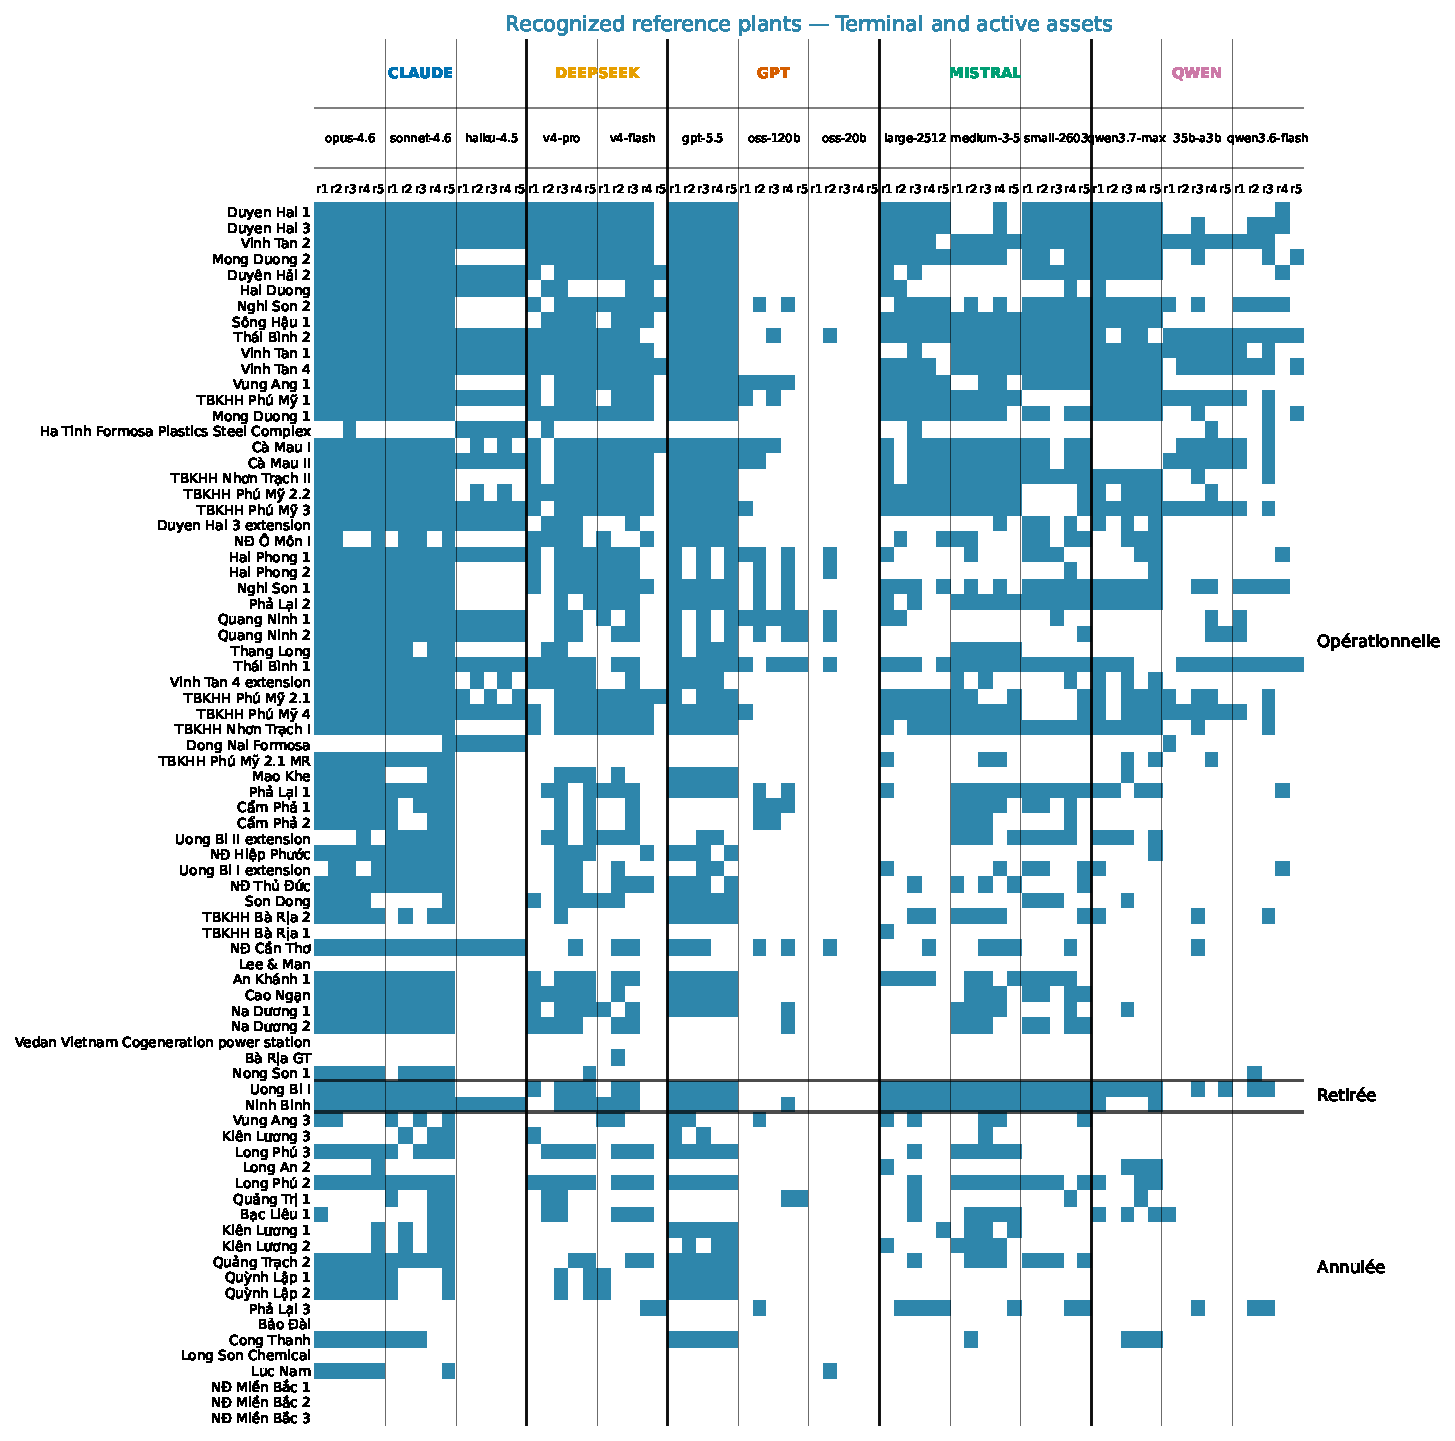
\includepdf[pages=-,pagecommand={\thispagestyle{plain}}]{inputs/generated/fig_exp1_recognition_matrix_portrait_fr.pdf}

% Auto-generated by aedist.tabulate_status_difficulty — do not edit
\begin{table}[htbp]
\centering
\caption{Composition de la liste de référence par statut, et taux de reconnaissance moyen (Expérience~1, méthode directe~: les 14~modèles à cinq répétitions). Le taux est la proportion de cellules (run~$\times$~centrale) reconnues parmi les centrales du statut. La liste est dominée par les centrales en projet, que la mémoire des modèles ne peut connaître.}\label{tab:status-difficulty}
\begin{tabular}{@{}lrrr@{}}
\toprule
Statut & $n$ & Part de la liste & Taux de reconnaissance \\
\midrule
En projet & 68 & 38.4\% & 8.4\% \\
Planifiée & 21 & 11.9\% & 29.7\% \\
En construction & 10 & 5.6\% & 44.9\% \\
Opérationnelle & 56 & 31.6\% & 45.2\% \\
Retirée & 2 & 1.1\% & 62.9\% \\
Annulée & 20 & 11.3\% & 15.4\% \\
\midrule
Ensemble & 177 & 100.0\% & 26.0\% \\
\bottomrule
\end{tabular}
\end{table}


% Glossaire — termes techniques utilisés dans le rapport
% Classé par domaine, alphabétique au sein de chaque domaine.

\chapter*{Glossaire}
\addcontentsline{toc}{chapter}{Glossaire}

\section*{Métriques d'évaluation}

\begin{description}
\item[Couverture] (\emph{recall, coverage}) Proportion des centrales de référence retrouvées par le système~: $\text{couverture} = \text{VP} / n_{\text{référence}}$. Mesure l'exhaustivité.
\item[F1 (score)] Moyenne harmonique de la précision et du rappel~: $\text{F1} = 2 \times \text{précision} \times \text{rappel} / (\text{précision} + \text{rappel})$. Métrique principale du benchmark, entre 0 et 1.
\item[Faux négatif (FN)] (\emph{false negative}) Centrale présente dans la référence mais absente de la sortie du système. Aussi appelée centrale \emph{manquante}.
\item[Faux positif (FP)] (\emph{false positive}) Centrale produite par le système mais absente de la référence. Voir \emph{hallucination}.
\item[Hallucination] Sortie du modèle ne correspondant à aucune entrée de la référence. Inclut les centrales inventées et les centrales non thermiques ajoutées à tort.
\item[Précision] (\emph{precision}) Proportion des centrales produites par le système qui sont correctes~: $\text{précision} = \text{VP} / n_{\text{système}}$.
\item[Vrai positif (VP)] (\emph{true positive}) Centrale correctement identifiée et appariée à la référence.
\end{description}

\section*{Méthodes et stratégies}

\begin{description}
\item[Agrégation multi-runs] (\emph{self-consistency}) Combinaison des résultats de plusieurs exécutions d'un même modèle pour réduire la variance. Le \emph{vote majoritaire} retient une centrale si elle apparaît dans 2+ runs sur 3~; l'\emph{union} retient une centrale si elle apparaît dans au moins 1 run.
\item[Chain of Thought] Technique de prompt incitant le modèle à détailler son raisonnement étape par étape avant de répondre.
\item[Décomposition] (\emph{decomposition}) Stratégie divisant une requête en sous-requêtes par type de combustible (charbon, gaz/GNL, pétrole/autres), puis fusionnant les résultats. Élimine la troncature.
\item[Few-shot learning] Technique de prompt fournissant quelques exemples de la réponse attendue pour guider le modèle.
\item[RAG (Retrieval Augmented Generation)] Enrichissement du contexte du modèle par injection de documents sources pertinents avant la requête.
\item[RAG wholesale] Variante injectant la totalité du corpus dans le message système, sans sélection de passages ni chunking.
\item[Réconciliation] (\emph{reconciliation}) Appariement des centrales produites par le système avec celles de la référence, par correspondance exacte et \emph{fuzzy matching}.
\item[Relance] (\emph{multi-turn, follow-up}) Approche conversationnelle avec messages de suivi pour inciter le modèle à compléter sa réponse.
\item[Requête directe] (\emph{single-shot}) Envoi d'un seul prompt au modèle, sans relance ni contexte additionnel. Méthode de référence.
\item[Self-consistency] Voir \emph{Agrégation multi-runs}.
\item[Sweep] (\emph{balayage}) Expérimentation à grande échelle paramétrant modèle $\times$ méthode $\times$ répétition.
\item[Vérification] (\emph{verification}) Post-traitement renvoyant la sortie au modèle (ou à un vérificateur indépendant) pour détecter les hallucinations.
\end{description}

\section*{Intelligence artificielle et infrastructure}

\begin{description}
\item[Deep Research] Mode d'interrogation des modèles de raisonnement (o3, DeepSeek~R1) avec budget de tokens élevé et recherche web intégrée.
\item[Embedding] (\emph{plongement}) Représentation vectorielle dense d'un texte, utilisée pour la recherche par similarité sémantique.
\item[Fenêtre de contexte] (\emph{context window}) Nombre maximal de tokens (entrée + sortie) qu'un modèle peut traiter en une requête.
\item[Fuzzy matching] (\emph{appariement flou}) Appariement approximatif de chaînes de caractères, tolérant les variations d'orthographe, d'accents et d'abréviations.
\item[LLM (Large Language Model)] Grand modèle de langage, réseau de neurones pré-entraîné sur de vastes corpus textuels.
\item[Modèle de raisonnement] (\emph{reasoning model}) LLM allouant une partie de son budget de tokens à un raisonnement explicite étape par étape (o3, o3-mini, DeepSeek~R1, QwQ).
\item[OCR (Optical Character Recognition)] Reconnaissance optique de caractères, conversion d'images ou de PDF scannés en texte.
\item[Open-weight] Modèle dont les poids sont publiés, permettant une exécution locale sans dépendance à un fournisseur cloud.
\item[Prompt] (\emph{invite}) Instruction textuelle envoyée au modèle. Versionnée et standardisée dans ce benchmark.
\item[Surgénération] (\emph{over-generation}) Régime d'erreur où le modèle produit plus de résultats que demandé, incluant des entrées hors du domaine (centrales non thermiques).
\item[Température] (\emph{temperature}) Paramètre de contrôle de l'aléa dans la génération~: 0 (déterministe) à 2 (forte variance). Fixée à 0 pour les sweeps direct\_complete et les bras paramétrique et livesearch de l'ablation~; non contrôlée (défaut fournisseur, typiquement~1,0) pour les sweeps direct, RAG, direct+multiturn, rag\_livesearch et rag\_per\_fuel. Voir section~\ref{sec:temperature-limitation}.
\item[Token] Unité d'encodage textuel utilisée par les LLM. Les tokens d'entrée (prompt) et de sortie (complétion) sont facturés séparément.
\item[Troncature] (\emph{truncation}) Coupure de la sortie du modèle avant complétion, due au dépassement de la limite de tokens. Principal facteur limitant en RAG wholesale.
\end{description}

\section*{Graphes de connaissances}

\begin{description}
\item[DBpedia] Base RDF extraite automatiquement de Wikipedia. Couverture variable, disponibilité intermittente.
\item[Graphe de connaissances] (\emph{knowledge graph}) Base de données structurée en triplets (sujet, prédicat, objet) reliant des entités et leurs propriétés.
\item[OEO (Open Energy Ontology)] Ontologie sémantique ouverte pour le domaine de l'énergie, définissant 15 types de centrales électriques.
\item[Ontologie] (\emph{ontology}) Modèle formel décrivant les concepts d'un domaine et leurs relations, servant de schéma au graphe de connaissances.
\item[OpenStreetMap (OSM)] Base de données géospatiale collaborative. Interrogée via l'API Overpass, elle retourne des centrales existantes avec coordonnées et périmètres.
\item[RDF (Resource Description Framework)] Standard W3C de représentation de la connaissance en triplets.
\item[Résolution d'entités] (\emph{entity resolution}) Processus associant les différentes mentions d'une même centrale (variantes de nom, translittérations) à une entité canonique.
\item[SPARQL] Langage de requête pour les bases de données RDF (Wikidata, DBpedia).
\item[Wikidata] Base de connaissances collaborative structurée, interrogeable via SPARQL.
\end{description}

\section*{Conversion de documents}

\begin{description}
\item[GROBID] Outil d'extraction de texte à partir de PDF, performant pour le texte courant mais aplatissant la structure tabulaire.
\item[Marker] Convertisseur PDF open-source. Meilleur résultat au benchmark~: 170 tableaux extraits avec diacritiques préservés.
\item[MinerU] Convertisseur PDF avec accélération GPU. Rapide (62 tableaux en 20~s) mais perd les diacritiques dans les cellules de tableaux.
\item[Mistral OCR] Backend OCR de Mistral, en accès direct via API. Extrait 169 tableaux sur le document de référence.
\end{description}

\section*{Domaine de l'énergie}

\begin{description}
\item[BOT (Build-Operate-Transfer)] Contrat de concession~: un investisseur construit et exploite une installation pendant une durée fixe, puis la transfère à l'État.
\item[CCGT (Combined Cycle Gas Turbine)] Centrale à gaz à cycle combiné, utilisant une turbine à gaz puis une turbine à vapeur pour un rendement d'environ 60\,\%.
\item[Centrale thermique] (\emph{thermal power plant}) Installation de production d'électricité par combustion (charbon, gaz, GNL, pétrole). Exclut l'hydraulique, l'éolien et le solaire.
\item[COD (Commercial Operation Date)] Date de mise en service commerciale d'une centrale, observée ou planifiée.
\item[Deep web] Partie du web non indexée par les moteurs de recherche~: documents administratifs, rapports institutionnels, bases de données non publiques.
\item[EVN (Vietnam Electricity Group)] Groupe national d'électricité du Vietnam (\emph{Tập đoàn Điện lực Việt Nam}).
\item[GNL (Gaz Naturel Liquéfié)] (\emph{LNG, Liquefied Natural Gas}) Gaz importé sous forme liquéfiée, par opposition au gaz naturel local.
\item[GW, MW, MWe] Unités de puissance électrique~: gigawatt ($10^3$~MW), mégawatt ($10^3$~kW), mégawatt électrique (distingue la puissance électrique de la puissance thermique MWth).
\item[PDP (Power Development Plan)] Plan de développement du secteur électrique du Vietnam. Versions~: PDP7 (2011), PDP7A, PDP8 (2021).
\item[SPV (Special Purpose Vehicle)] Entité juridique dédiée à la propriété ou l'exploitation d'une installation. Souvent un consortium multinational.
\end{description}


\bibliography{refs}

\end{document}
